\documentclass[11pt,a4paper]{article}

\usepackage[utf8]{inputenc}
\usepackage{microtype}
\usepackage[margin=1in]{geometry}
\usepackage{amsmath,amssymb,amsthm,mathtools,cancel}
\usepackage{booktabs}
\usepackage{array}
\usepackage{multirow}
\usepackage{enumitem}
\usepackage{xcolor}
\usepackage{graphicx}
\usepackage{tikz}
\usetikzlibrary{arrows.meta,positioning,calc,decorations.pathreplacing}
\usepackage{hyperref}

\definecolor{accentred}{RGB}{178, 24, 43}

\hypersetup{
    colorlinks=true,
    linkcolor=blue!60!black,
    citecolor=blue!60!black,
    urlcolor=blue!60!black,
    pdftitle={Primal-Shortened ISD Key Recovery on Binary Goppa Codes},
    pdfauthor={MiniMax}
}

\newtheorem{theorem}{Theorem}
\newtheorem{lemma}{Lemma}
\newtheorem{proposition}{Proposition}
\newtheorem{corollary}{Corollary}
\theoremstyle{definition}
\newtheorem{definition}{Definition}
\theoremstyle{remark}
\newtheorem{remark}{Remark}

\newcommand{\F}{\mathbb{F}}
\newcommand{\Z}{\mathbb{Z}}
\newcommand{\R}{\mathbb{R}}
\newcommand{\wt}{\operatorname{wt}}
\newcommand{\supp}{\operatorname{supp}}
\newcommand{\rk}{\operatorname{rank}}
\newcommand{\diag}{\operatorname{diag}}
\newcommand{\Cat}{\operatorname{Cat}}
\newcommand{\RREF}{\operatorname{RREF}}
\newcommand{\ISD}{\mathsf{ISD}}
\newcommand{\BJMM}{\mathsf{BJMM}}
\newcommand{\HOV}{\mathsf{HOV}}
\newcommand{\HOVER}{\mathsf{HOVER}}

\title{\textbf{Primal-Shortened ISD Key Recovery on Binary Goppa Codes}}
\author{MiniMax}
\date{November 2026}

\begin{document}
\maketitle

\begin{abstract}
Binary Goppa codes form the algebraic foundation of the McEliece cryptosystem and the NIST post-quantum candidate Classic McEliece. To evaluate concrete key-recovery security margins across code parameters, the Technology Innovation Institute (TII) McEliece Challenges provide $206$ structural key-recovery instances (Track~2). Existing algebraic key-recovery attacks rely either on shortened-dual rank-$2$ and higher-order vanishing ($\HOV/\HOVER$) systems, whose standard kernels collapse at moderate code rates, or on primal hold-out attacks, whose high-order derivative systems still span up to tens of millions of columns after shortening.

We present a primal-shortened key-recovery framework (Route~A) built on a direct structural observation: although the public parity-check matrix scrambles the rows of the private Goppa matrix, it leaves the primal codeword space invariant, where every minimum-weight codeword obeys an exact quadratic identity over the secret support. Restricting the primal code to a compact column window before sampling compresses this degree-$2$ interpolation system by up to $6.59\times$ without penalizing multi-target Information-Set Decoding ($\ISD$) yield. Pairing a cache-resident multi-target $\ISD$ engine with a systematic $\F_2$-linear lifting solver reduces key recovery to lightweight codeword harvesting plus seconds of dense binary linear algebra, complemented by an accelerated $\HOVER$ solver (Route~B) on one high-rate parameter family.

Across the official TII catalog, our framework recovers $94$ Track-2 private keys ($89$ via Route~A and $5$ via Route~B), achieving $55$ first-blood recoveries and accelerating $39$ previously solved instances, with all $94$ keys verified by TII's official SageMath checker. Compared to the shortened-dual records on \texttt{TII-166} and \texttt{TII-125} ($9.20\text{ h}$ and $9.47\text{ h}$ on $72$ cores, CRYPTO~2026), Route~A finishes in $5.36\text{ s}$ and $5.90\text{ s}$ on a single $64$-core CPU server, achieving $6{,}968\times$ and $6{,}493\times$ core-hour speedups. On \texttt{TII-254} and \texttt{TII-253}, it finishes in $30.4\text{ s}$ and $1.80\text{ s}$, achieving $1{,}896\times$ and $43{,}400\times$ wall-time speedups over the prior GPU-cluster record and the multi-core hold-out record by Anthropic. Finally, our codeword-supply analysis shows that Classic McEliece standard parameters lie far outside the feasible regime of this attack.
\end{abstract}

\section{Introduction}
\label{sec:intro}

Code-based public-key cryptography, initiated by McEliece~\cite{McE78} in 1978 and reformulated in dual syndrome form by Niederreiter~\cite{Nie86}, is one of the oldest approaches to public-key encryption that resists quantum attacks. Its security rests on two distinct assumptions: the average-case hardness of bounded-distance syndrome decoding in random binary linear codes (whose worst-case general decoding problem is NP-complete~\cite{BMvT78}), and the structural hardness of distinguishing a public Goppa parity-check matrix $H_{\text{pub}} \in \F_2^{mt \times n}$ from a uniform matrix or recovering its secret algebraic representation. Whereas high-rate alternant instances and compact algebraic proposals such as generalized Reed--Solomon subcodes succumbed to structural distinguishers and filtration attacks~\cite{FGOPT13,CGGOT14}, binary Goppa codes~\cite{Pat75,MS77} have withstood nearly five decades of cryptanalysis and form the basis of the NIST post-quantum key-encapsulation candidate Classic McEliece.

To benchmark the concrete complexity of code-based cryptanalysis across code lengths $n$, extension degrees $m = [\F_{2^m} : \F_2]$, and Goppa degrees $t$, Kirshanova and Esser~\cite{KE23} introduced the TII McEliece Challenges, organized into three tracks:\footnote{We follow the Track~1--3 numbering of the challenge repository~\cite{KE23}, corresponding on the HeroX portal to Track~1A (theoretical key recovery), Track~1B (practical key recovery), and Tracks~2A--2B (message recovery).}
\begin{enumerate}[leftmargin=2em]
    \item \textbf{Theoretical Key-Recovery Algorithms (Track~1):}
    Design classical or quantum key-recovery and distinguishing algorithms with improved asymptotic or concrete complexity in secure McEliece parameter regimes. Because this track evaluates algorithmic designs rather than fixed public keys, no challenge files are generated for Track~1 in the companion repository~\cite{KE23}.
    \item \textbf{Practical Structural Key Recovery (Track~2):}
    Given \emph{only} a concrete public parity-check matrix $H_{\text{pub}} \in \F_2^{mt \times n}$ and the field polynomial $f(x)$ defining $\F_q = \F_2[x]/(f(x))$ ($q = 2^m$), recover a support tuple $\hat{L} = (\hat{z}_0, \dots, \hat{z}_{n-1}) \in \F_q^n$ of $n$ distinct elements and a monic square-free degree-$t$ Goppa polynomial $\hat{g}(X) \in \F_q[X]$ ($\hat{g}(\hat{z}_j) \neq 0$; chosen irreducible in TII's generator~\cite{KE23}) whose vertical $\F_2$-expansion $H_{\text{raw}}(\hat{L}, \hat{g}) \in \F_2^{mt \times n}$ of the alternant matrix $\big(\hat{z}_j^i / \hat{g}(\hat{z}_j)\big)_{0 \le i < t,\, 0 \le j < n}$ reproduces the public key in reduced row-echelon form:
    \begin{equation}
    \label{eq:intro-rref}
        \RREF\!\big(H_{\text{raw}}(\hat{L}, \hat{g})\big) = H_{\text{pub}}.
    \end{equation}
    \item \textbf{Practical Syndrome Decoding (Track~3):}
    Given $H_{\text{pub}} \in \F_2^{mt \times n}$ and a target syndrome $s = H_{\text{pub}} e^\top \in \F_2^{mt}$ for an unknown weight-$t$ error vector $e \in \F_2^n$, recover $e$. Treating $H_{\text{pub}}$ as a generic binary linear code, this problem is the domain of single-target \emph{Information-Set Decoding ($\ISD$)} and code-sieving algorithms, spanning Lee--Brickell~\cite{LB88}, Stern--Dumer~\cite{Ste88,Dum91}, Canteaut--Chabaud~\cite{CC98}, Ball-Collision~\cite{BLP11}, multi-layer representation ($\BJMM$) and nearest-neighbor decoders~\cite{MMT11,BJMM12,MO15}, and recent advances in code sieving, dual reductions, and concrete cost modeling~\cite{DEEK24,CDMT24,BC24}.
\end{enumerate}
Throughout this paper, we study the $206$ concrete key-recovery instances of Track~2.

\subsection{Prior Key-Recovery Paradigms and Bottlenecks}
The $206$ Track-2 challenges span extension degrees $m \in \{5, \dots, 10\}$, Goppa degrees $t \in \{2, \dots, 24\}$, and security ratings $\lambda_{\text{TII}} \in [22, 255]$. The $36$ instances with $\lambda_{\text{TII}} \le 82$ were solved during the initial competition without published keys, while $41$ of the $170$ instances with $\lambda_{\text{TII}} \ge 83$ were subsequently solved across eight public papers and repositories~\cite{Pan25,BLT26,BLRT26,Hem26,Ved26,Saa26a,Saa26b,SaaRepo,Wei26}. Aside from Panny's support-splitting search on small parameters~\cite{Pan25} (such as $161$ core-days on \texttt{TII-91}), published algebraic key-recovery attacks fall into two paradigms.

\paragraph{Shortened-Dual Rank-$2$ and Higher-Order Vanishing Attacks.}
Because the rows of $H_{\text{raw}}(L, g)$ are $\F_2$-bit slices of rational evaluations $z_j^i / g(z_j)$ over $\F_{2^m}$, componentwise products of dual codewords satisfy low-rank polynomial relations that do not hold for random linear codes. Building on high-rate alternant distinguishers~\cite{FGOPT13,CGGOT14}, quadratic-form spaces~\cite{CMT23}, the syzygy distinguisher~\cite{Ran25}, and the higher-order vanishing ($\HOV$) distinguisher~\cite{HW26}, recent attacks first shorten the dual code $\Gamma(L, g)^\perp$ at $s$ coordinates to compress its dimension before extracting algebraic structure. Bardet, Lemoine, and Tillich~\cite{BLT26} (via Pfaffian rank-$2$ ideals) and Briaud et al.~\cite{BLRT26} (via bilinear rank-$2$ modeling) isolate rank-$2$ forms in the shortened dual square, whereas Hemmert~\cite{Hem26} (via low-rank catalecticant MinRank search) and Saarinen~\cite{Saa26a} ($\HOVER$, via the public $\F_{2^m}$-endomorphism algebra) exploit degree-$3$ and degree-$4$ forms that vanish together with all first partial derivatives on the shortened dual code. Although these dual methods account for $37$ of the $41$ prior Track-2 solutions, their non-trivial vanishing kernels exist only at high code rates and collapse once $R = k/n$ drops toward or below $1 - 2/t$. Even near this boundary, solving the resulting polynomial or MinRank systems required up to $9.47\text{ h}$ and $223\text{ GB}$ RAM on $72$ Xeon cores (\texttt{TII-125}~\cite{BLT26}, CRYPTO~2026) or $47.75\text{ h}$ on $256$ EPYC cores (\texttt{TII-223}~\cite{Hem26}).

\paragraph{Primal Hold-Out Attacks.}
To reach moderate code rates where shortened-dual kernels vanish, Ghoshal, Ishai, Jain, and Sun~\cite{GIJS26} introduced the primal \emph{hold-out distinguisher}, which Vedenev~\cite{Ved26}, Weis~\cite{Wei26}, and Saarinen~\cite{Saa26b} extended to key recovery. Viewing the columns of a shortened generator matrix (of dimension $k_\ell \in [35, 50]$) as points on a hidden rational curve, the attack holds out one or two anchor columns and searches for low-degree $k_\ell$-variate polynomials (typically of degree~$6$) whose values and low-order Hasse derivatives vanish at all remaining columns. By univariate Hermite interpolation along the curve, any such polynomial must also vanish at the held-out columns, exposing the secret support inside the kernel. However, representing degree-$6$ multilinear polynomials in $k_\ell$ variables still produces sparse matrices of width $\binom{k_\ell}{6} \sim 10^7$ columns, turning kernel extraction into a large-scale sparse Krylov or block-Lanczos computation. Recovering \texttt{TII-253} $(214, 8, 9)$ took $21.7\text{ h}$ on $32$ Xeon threads by Weis at Anthropic~\cite{Wei26} or $14.0\text{ h}$ on an H200 GPU with $48$ CPU threads~\cite{Ved26} (which also solved the shorter instances \texttt{TII-173} and \texttt{TII-249}). Scaling further to \texttt{TII-254} $(223, 8, 12)$ required two deflated $15{,}527{,}170$-column operators taking $16.0\text{ h}$ wall time and $128\text{ GiB}$ RAM on up to $8\times$ NVIDIA GH200 GPUs ($27.2\text{ GH200 GPU-h}$ across the two Krylov stages)~\cite{Saa26b,SaaRepo}.

\begin{table}[t]
\centering
\caption{Flagship key-recovery comparison on TII Track-2 challenges across wall-clock runtime, compute cost, and peak memory.}
\label{tab:comparison}
{\footnotesize
\setlength{\tabcolsep}{3.2pt}
\renewcommand{\arraystretch}{1.10}
\resizebox{\textwidth}{!}{\begin{tabular}{@{}llcccccl@{}}
\toprule
\textbf{ID} & \textbf{Parameters} & \textbf{Prior Time} & \textbf{Prior Compute} & \textbf{Our Time} & \textbf{Our Compute} & \textbf{RAM} & \textbf{Speedup / Status} \\
\midrule
\texttt{83}  & $(253, 8, 5, 213)$    & $24.3\text{ s}$~\cite{SaaRepo}        & $0.081\text{ ch}$ ($12\text{ cores}$)   & $\mathbf{1.58\text{ s}}$  & $\mathbf{0.028\text{ ch}}$ & $232\text{ MB}$  & $15.4\times$ time / $2.9\times$ ch \\
\texttt{125} & $(507, 9, 7, 444)$    & $9.47\text{ h}$~\cite{BLT26}          & $681.8\text{ ch}$ ($72\text{ cores}$)   & $\mathbf{5.90\text{ s}}$  & $\mathbf{0.105\text{ ch}}$ & $340\text{ MB}$  & $5{,}778\times$ time / $6{,}493\times$ ch \\
\texttt{166} & $(500, 9, 7, 437)$    & $9.20\text{ h}$~\cite{BLT26}          & $662.5\text{ ch}$ ($72\text{ cores}$)   & $\mathbf{5.36\text{ s}}$  & $\mathbf{0.095\text{ ch}}$ & $340\text{ MB}$  & $6{,}180\times$ time / $6{,}968\times$ ch \\
\texttt{210} & $(491, 9, 7, 428)$    & $4.31\text{ h}$~\cite{BLT26}          & $310.2\text{ ch}$ ($72\text{ cores}$)   & $\mathbf{6.04\text{ s}}$  & $\mathbf{0.107\text{ ch}}$ & $340\text{ MB}$  & $2{,}568\times$ time / $2{,}899\times$ ch \\
\texttt{253} & $(214, 8, 9, 142)$    & $21.7\text{ h}$~\cite{Wei26}          & $694.4\text{ th}$ ($32\text{ threads}$) & $\mathbf{1.80\text{ s}}$  & $\mathbf{0.032\text{ ch}}$ & $242\text{ MB}$  & $43{,}400\times$ time / $21{,}688\times$ th \\
\texttt{253} & $(214, 8, 9, 142)$    & $14.0\text{ h}$~\cite{Ved26}          & $1{\times}\text{H200}+48\text{ threads}$ & $\mathbf{1.80\text{ s}}$  & $\mathbf{0.032\text{ ch}}$ & $242\text{ MB}$  & $28{,}000\times$ time (CPU vs.\ GPU) \\
\texttt{223} & $(492, 9, 9, 411)$    & $47.75\text{ h}$~\cite{Hem26}         & $12{,}224\text{ ch}$ ($256\text{ cores}$) & $\mathbf{39.9\text{ s}}$ & $\mathbf{0.709\text{ ch}}$ & $326\text{ MB}$  & $4{,}308\times$ time / $17{,}241\times$ ch \\
\texttt{129} & $(509, 9, 9, 428)$    & $4.51\text{ h}$~\cite{Saa26a}         & $126.2\text{ vch}$ ($28\text{ vCPUs}$)  & $\mathbf{41.3\text{ s}}$  & $\mathbf{0.734\text{ ch}}$ & $340\text{ MB}$  & $393\times$ time / $172\times$ vch \\
\texttt{213} & $(496, 9, 10, 406)$   & $6.74\text{ h}$~\cite{Saa26a}         & $188.8\text{ vch}$ ($28\text{ vCPUs}$)  & $\mathbf{138.8\text{ s}}$ & $\mathbf{2.47\text{ ch}}$  & $358\text{ MB}$  & $175\times$ time / $76.5\times$ vch \\
\texttt{254} & $(223, 8, 12, 127)$   & $16.0\text{ h}$~\cite{Saa26b,SaaRepo} & $8{\times}\text{GH200}$ ($27.2\text{ GPU-h}^\ast$) & $\mathbf{30.4\text{ s}}$ & $\mathbf{0.540\text{ ch}}$ & $313\text{ MB}$ & $1{,}896\times$ time (CPU vs.\ GPU) \\
\texttt{252} & $(1008, 10, 11, 898)$ & $375\text{ s}$~\cite{Saa26a}          & $1.25\text{ ch}$ ($12\text{ cores}$)    & $\mathbf{90.0\text{ s}}$  & $\mathbf{0.025\text{ ch}}$ & $1.45\text{ GB}$ & $4.17\times$ time / $50.0\times$ ch \\
\midrule
\texttt{147} & $(509, 9, 11, 410)$   & \multicolumn{2}{c}{\emph{No prior published solution}}                  & $\mathbf{408\text{ s}}$   & $\mathbf{7.25\text{ ch}}$  & $373\text{ MB}$  & \textbf{First-Blood} ($n'=303$) \\
\texttt{232} & $(233, 8, 13, 129)$   & \multicolumn{2}{c}{\emph{No prior published solution}}                  & $\mathbf{332\text{ s}}$   & $\mathbf{5.90\text{ ch}}$  & $254\text{ MB}$  & \textbf{First-Blood} ($n'=233$) \\
\texttt{245} & $(493, 9, 12, 385)$   & \multicolumn{2}{c}{\emph{No prior published solution}}                  & $\mathbf{2510\text{ s}}$  & $\mathbf{44.62\text{ ch}}$ & $422\text{ MB}$  & \textbf{First-Blood} ($n'=326$) \\
\texttt{172} & $(1020, 10, 11, 910)$ & \multicolumn{2}{c}{\emph{No prior published solution}}                  & $\mathbf{89.9\text{ s}}$  & $\mathbf{0.025\text{ ch}}$ & $1.51\text{ GB}$ & \textbf{First-Blood} (Route~B) \\
\texttt{165} & $(251, 8, 14, 139)$   & \multicolumn{2}{c}{\emph{No prior published solution}}                  & $\mathbf{81.2\text{ s}}$  & $\mathbf{1.44\text{ ch}}$  & $263\text{ MB}$  & \textbf{First-Blood} ($n'=250$) \\
\texttt{250} & $(1010, 10, 12, 890)$ & \multicolumn{2}{c}{\emph{No prior published solution}}                  & $\mathbf{9.20\text{ h}}^\dagger$  & $\mathbf{66{,}722\text{ ch}}^\dagger$ & $1.28\text{ GB}$ & \textbf{First-Blood} ($n'=467$) \\
\texttt{228} & $(500, 9, 14, 374)$   & \multicolumn{2}{c}{\emph{No prior published solution}}                  & $\mathbf{57.1\text{ min}}^\dagger$ & $\mathbf{2{,}463\text{ ch}}^\dagger$  & $468\text{ MB}$  & \textbf{First-Blood} ($n'=361$) \\
\bottomrule
\end{tabular}}
\\[0.35em]
\parbox{\textwidth}{\footnotesize
\emph{Notes:} Parameters are $(n, m, t, k)$; $\text{ch}$, $\text{th}$, and $\text{vch}$ denote physical core-hours ($64$ Xeon cores for Route~A, $1$ core for Route~B), thread-hours~\cite{Wei26}, and vCPU-hours~\cite{Saa26a}. $^\ast$$16.0\text{ h}$ wall is from~\cite{SaaRepo} and $27.2\text{ GPU-h}$ in~\cite{Saa26b} covers the two Krylov runs; $^\dagger$cluster runs ($2{,}048\text{--}10{,}240$ EPYC cores).}}
\end{table}

\subsection{Main Results and Technical Overview}
Our primary method (Route~A) bypasses both the dual rate barrier and multi-million-column hold-out matrices by working directly with \emph{minimum-weight codewords of a shortened primal code}. Although the RREF transformation $H_{\text{pub}} = T^{-1} H_{\text{raw}}(L, g)$ scrambles the rows of the parity-check matrix, the primal code $\Gamma(L, g) = \ker_{\F_2}(H_{\text{pub}})$ is unchanged. In characteristic~$2$, differentiating the support locator polynomial $\sigma_S(X) = \prod_{j \in S}(X - z_j)$ of any minimum odd-weight codeword ($w = 2t + 1$) annihilates odd elementary symmetric functions and yields the exact polynomial square $\sigma'_S(X) = \bar{g}(X)^2$~\cite{Pat75,MS77,Fin03} (Theorem~\ref{thm:deriv-square}). Matching its $X^{2t-2}$ coefficient gives the constant quadratic identity
\begin{equation}
\label{eq:intro-e2}
    e_2(z_S) = \sum_{0 \le u < v < n} c_u c_v\, z_u z_v = \bar{g}_{t-1}^2 \in \F_q.
\end{equation}
Expanding~\eqref{eq:intro-e2} into $m$ coordinate bits over $\F_2$ turns every weight-$(2t+1)$ codeword $c$ into $m$ binary quadratic equations over the secret support products $z_u z_v$. Route~A turns this identity into a fast key-recovery engine via two pairs of techniques:
\begin{itemize}[leftmargin=1.5em]
    \item \textbf{Primal Shortening and Cache-Resident Multi-Target $\ISD$ (Section~\ref{sec:isd-shortening}):}
    Restricting $H_{\text{pub}}$ to a window of $n' \ll n$ columns preserves the Goppa polynomial $g(X)$ while compressing the number of quadratic interpolation unknowns $F(d) = \Theta((n' - mt)^2)$ by up to $6.59\times$. Because multi-target $\ISD$ harvests \emph{any} $F(d)$ distinct weight-$(2t+1)$ codewords from the shortened pool, the $\binom{n'}{w}$ pool-size factor cancels the $\binom{n'}{w}$ denominator of the single-word $\ISD$ capture probability (Proposition~\ref{prop:isd-cancellation}). Furthermore, in the shortened multi-core regime, keeping single-stage Ball-Collision and L1d-bitmap-filtered Stern--Dumer tables inside per-core L1d/L2 caches avoids the DRAM bandwidth bottleneck of multi-layer $\BJMM$.
    \item \textbf{Public Polarization Quotient and Systematic $\F_2$-Linear Lifting (Section~\ref{sec:algebraic-lifting}):}
    After restricting to the odd-weight affine hyperplane and quotienting out the public combinatorial identity $\sum_{u<v} c_u c_v = \binom{2t+1}{2} \equiv t \pmod 2$ (Theorem~\ref{thm:shortened-lift}), we transform the affine generator into systematic form $[I_d \mid P]$. This traps all $d$ pivot diagonal weights on the main diagonal of the rank-$m$ target matrices, allowing us to recover the shortened support $L_A$, extract $\bar{g}(X) = \sqrt{\sigma'_S(X)}$ from a single codeword, and extend $L_A$ to all $n$ columns via $O(n)$ closed-form field divisions without Gröbner bases.
\end{itemize}
For the single high-rate family $(m,t)=(10,11)$, we pair Route~A with a Frobenius-reduced shortened-dual $\HOVER$ solver (Route~B, summarized in Section~\ref{subsec:route-b-summary} and detailed in Appendix~\ref{app:route-b}).

As summarized in Table~\ref{tab:comparison} and Section~\ref{sec:experiments}, our framework solves $94$ official TII Track-2 challenges (\texttt{TII-83} through \texttt{TII-254}), achieving $55$ first-blood recoveries (including \texttt{TII-133}, \texttt{TII-228} at $mt=126$, and \texttt{TII-250} at $mt=120$) and accelerating $39$ published instances, with all $94$ keys passing TII's official SageMath verification script ($94/94$ verified). The $92$ single-node instances finish in $177.82$ physical core-hours combined.

\section{Binary Goppa Codes and Minimum-Weight Structure}
\label{sec:prelim}

\subsection{Public-Key Construction over \texorpdfstring{$\F_{2^m}$}{F\_\{2\^m\}}}
Fix an extension degree $m \ge 1$ and field size $q = 2^m$, with $\F_q = \F_2[x]/(f(x))$ defined by a degree-$m$ irreducible polynomial $f(x) \in \F_2[x]$ and primitive root $a = x \bmod f(x)$. Every element $\alpha = \sum_{b=0}^{m-1} c_b a^b \in \F_q$ has a dual representation:
\begin{itemize}[leftmargin=1.5em]
    \item \textbf{Field scalar in $\F_q$:} $\alpha$ supports finite-field arithmetic and polynomial evaluation; in characteristic~$2$, $-1 = +1$, $(A + B)^2 = A^2 + B^2$, and the Frobenius squaring map $\alpha \mapsto \alpha^2$ is an automorphism with unique square-root inverse $\sqrt{\alpha} = \alpha^{2^{m-1}}$.
    \item \textbf{Bit vector in $\F_2^m$:} Via the $\F_2$-vector space isomorphism $\phi: \F_q \to \F_2^m$ mapping $\sum_{b=0}^{m-1} c_b a^b \mapsto (c_0, c_1, \dots, c_{m-1})^\top$, $\alpha$ is a vertical column vector of $m$ bits.
\end{itemize}

In the official TII specification~\cite{KE23}, the public key $H_{\text{pub}}$ is generated from the private key $(L, g)$ in three steps:

\begin{definition}[Binary Goppa Public-Key Construction]
\label{def:goppa}
Let $L = (z_0, z_1, \dots, z_{n-1}) \in \F_q^n$ be an ordered tuple of $n \le q$ pairwise distinct support elements, and let $g(X) = \sum_{i=0}^t g_i X^i \in \F_q[X]$ be a square-free Goppa polynomial of degree $t \ge 2$ satisfying $g(z_j) \neq 0$ for all $0 \le j < n$ (chosen monic irreducible in TII's generator~\cite{KE23} and Classic McEliece).
\begin{enumerate}[leftmargin=2em]
    \item \textbf{Step 1: Weighted Vandermonde Parity-Check Matrix over $\F_q$.}
    Form the $t \times n$ alternant parity-check matrix $H_{\F_q}(L, g) \in \F_q^{t \times n}$ with entries
    \begin{equation}
    \label{eq:h-fq}
        H_{\F_q}(L, g)_{i, j} = \frac{z_j^i}{g(z_j)} \qquad (0 \le i < t,\; 0 \le j < n),
    \end{equation}
    explicitly written as
    \[
        H_{\F_q}(L, g) =
        \begin{pmatrix}
            \dfrac{1}{g(z_0)} & \dfrac{1}{g(z_1)} & \cdots & \dfrac{1}{g(z_{n-1})} \\[0.8em]
            \dfrac{z_0}{g(z_0)} & \dfrac{z_1}{g(z_1)} & \cdots & \dfrac{z_{n-1}}{g(z_{n-1})} \\[0.4em]
            \vdots & \vdots & \ddots & \vdots \\[0.4em]
            \dfrac{z_0^{t-1}}{g(z_0)} & \dfrac{z_1^{t-1}}{g(z_1)} & \cdots & \dfrac{z_{n-1}^{t-1}}{g(z_{n-1})}
        \end{pmatrix} \in \F_q^{t \times n}.
    \]
    \item \textbf{Step 2: Vertical $m$-Bit Expansion into $\F_2^{mt \times n}$.}
    Expand each entry $H_{\F_q}(L, g)_{i, j} \in \F_q$ vertically into an $m$-bit column vector via $\phi: \F_q \to \F_2^m$, producing the raw binary parity-check matrix $H_{\text{raw}}(L, g) \in \F_2^{mt \times n}$:
    \begin{equation}
    \label{eq:h-raw}
        H_{\text{raw}}(L, g)_{mi + b, j} = \phi\!\left(\frac{z_j^i}{g(z_j)}\right)_{\!b} \qquad (0 \le i < t,\; 0 \le b < m,\; 0 \le j < n).
    \end{equation}
    The \emph{binary Goppa code} $\Gamma(L, g) \subseteq \F_2^n$ is the binary right kernel of this matrix:
    \begin{equation}
    \label{eq:goppa-kernel}
        \Gamma(L, g) \coloneqq \big\{c \in \F_2^n : H_{\F_q}(L, g)\,c^\top = 0 \text{ in } \F_q^t\big\}
        = \ker_{\F_2}\!\big(H_{\text{raw}}(L, g)\big).
    \end{equation}
    \item \textbf{Step 3: Row-Scrambling via RREF.}
    When $H_{\text{raw}}(L, g)$ has full row rank $mt$, the code has dimension $k = n - mt$. Key generation applies Gaussian elimination over $\F_2$ and publishes only the canonical reduced row-echelon form
    \begin{equation}
    \label{eq:h-pub}
        H_{\text{pub}} = \RREF\!\big(H_{\text{raw}}(L, g)\big) = T^{-1} H_{\text{raw}}(L, g) \in \F_2^{mt \times n},
    \end{equation}
    where $T \in \mathrm{GL}_{mt}(\F_2)$ is the secret invertible $mt \times mt$ binary row-mixing matrix determined by the $mt$ pivot columns of $H_{\text{raw}}(L, g)$ (for systematic instances, $H_{\text{pub}} = [I_{mt} \mid R]$).
\end{enumerate}
\end{definition}

\subsection{Row Scrambling and Codeword Space Invariance}
If an attacker were given the unscrambled matrix $H_{\text{raw}}(L, g)$ prior to Step~3, regrouping the first $m$ rows of column $j$ would yield $v_{0, j} = 1 / g(z_j) \in \F_q^\times$ and regrouping rows $m$ through $2m - 1$ would yield $v_{1, j} = z_j / g(z_j) \in \F_q$. Their ratio immediately reveals every support element in $O(n)$ field divisions:
\begin{equation}
\label{eq:direct-ratio}
    z_j = \frac{v_{1, j}}{v_{0, j}} = \frac{z_j / g(z_j)}{1 / g(z_j)} \qquad (0 \le j < n),
\end{equation}
after which $g(X)$ follows by linear interpolation from $g(z_j) = 1 / v_{0, j}$.

On the public key $H_{\text{pub}} = T^{-1} H_{\text{raw}}(L, g)$, however, the unknown matrix $T^{-1} \in \mathrm{GL}_{mt}(\F_2)$ takes arbitrary $\F_2$-linear combinations across all $mt$ binary rows, mixing the $b$-th bit of $1 / g(z_j)$ with the $b'$-th bit of $z_j^{t-1} / g(z_j)$. Individual rows of $H_{\text{pub}}$ no longer group into coherent $m$-bit field elements, and brute-forcing $T \in \mathrm{GL}_{mt}(\F_2)$ costs $\approx 2^{(mt)^2}$. (Note that any column permutation $P$ of $H_{\text{raw}}(L, g)$ merely reorders the support tuple $L \mapsto L P$, so $T^{-1}$ is the sole algebraic barrier between $H_{\text{pub}}$ and $(L, g)$.)

Left-multiplying by an invertible matrix $T^{-1} \in \mathrm{GL}_{mt}(\F_2)$ leaves the right kernel completely invariant:
\begin{equation}
\label{eq:kernel-invariance}
    c \in \Gamma(L, g)
    \iff H_{\text{raw}}(L, g)\,c^\top = 0
    \iff T^{-1} H_{\text{raw}}(L, g)\,c^\top = H_{\text{pub}}\,c^\top = 0.
\end{equation}
Every codeword $c \in \ker_{\F_2}(H_{\text{pub}})$ is therefore unaffected by $T^{-1}$ and obeys the exact algebraic identities of $H_{\F_q}(L, g)$. Moreover, for any affine automorphism $z \mapsto \alpha z + \beta$ ($\alpha \in \F_q^\times, \beta \in \F_q$) and Frobenius power $\sigma \in \operatorname{Gal}(\F_q/\F_2)$, transforming $(L, g)$ to $(\alpha L^\sigma + \beta,\, \alpha^t g^\sigma(\alpha^{-1}(X - \beta)))$ preserves the binary parity-check row space and keeps $g$ monic; any such equivalent key $(\hat{L}, \hat{g})$ satisfies~\eqref{eq:intro-rref}.

\subsection{Minimum-Weight Locator Derivative Identity}
To connect $\ker_{\F_2}(H_{\text{pub}})$ to $(L, g)$, observe that for each $j \in \{0, \dots, n-1\}$, the polynomial $g(X) - g(z_j)$ is divisible by $X - z_j$ with degree-$(t-1)$ quotient $\sum_{i=0}^{t-1} g_{i+1}\sum_{r=0}^i z_j^r X^{i-r}$. Hence, in $\F_q[X]/(g(X))$,
\[
    \frac{1}{X - z_j} \equiv -\frac{g(X) - g(z_j)}{g(z_j)(X - z_j)} \pmod{g(X)}.
\]
Summing over $j = 0, \dots, n-1$ weighted by $c_j \in \{0, 1\}$ shows that the $t$ field parity checks $\sum_{j=0}^{n-1} c_j z_j^i / g(z_j) = 0$ ($0 \le i < t$) are equivalent to the classical \emph{Goppa syndrome condition}~\cite{Pat75,MS77}:
\begin{equation}
\label{eq:goppa-syndrome}
    S_c(X) \coloneqq \sum_{j=0}^{n-1} \frac{c_j}{X - z_j} = \sum_{j \in S} \frac{1}{X - z_j} \equiv 0 \pmod{g(X)},
\end{equation}
where $S = \supp(c) = \{j \in \{0, \dots, n-1\} : c_j = 1\}$ and $w = |S| = \wt(c)$. Define the \emph{support locator polynomial} of $c$:
\begin{equation}
\label{eq:locator-def}
    \sigma_S(X) \coloneqq \prod_{j \in S} (X - z_j) = \sum_{i=0}^w e_i(z_S)\, X^{w - i} \in \F_q[X],
\end{equation}
where $e_i(z_S) = \sum_{J \subseteq S, |J|=i} \prod_{j \in J} z_j$ is the $i$-th elementary symmetric polynomial of the active support elements $z_S = (z_j)_{j \in S}$ (since $-1 = +1$ in $\F_q$). Let $\bar{g}(X) = g(X) / g_t = X^t + \sum_{i=0}^{t-1} \bar{g}_i X^i$ denote the monic normalization of $g(X)$. In binary square-free Goppa codes, divisibility $\bar{g}(X)^2 \mid \sigma'_S(X)$ yields $d_{\min} \ge 2t + 1$~\cite{Pat75,MS77}, and Finiasz~\cite{Fin03} observed that at minimum weight $w = 2t + 1$ monic degree equality forces $\sigma'_S(X) = \bar{g}(X)^2$ (fixing all even elementary symmetric coefficients of $\sigma_S(X)$ when $(L, g)$ is known; see~\cite{Ved26,Wei26} for higher-order differential identities on general codewords). Route~A exploits the $X^{2t-2}$ coefficient of this classical identity in the inverse direction to build quadratic key-recovery equations over unknown $(L, g)$:

\begin{theorem}[Minimum-Weight Locator Derivative Identity]
\label{thm:deriv-square}
Let $\Gamma(L, g)$ be a binary Goppa code with square-free degree-$t$ Goppa polynomial $g(X)$ and monic normalization $\bar{g}(X) = X^t + \sum_{i=0}^{t-1} \bar{g}_i X^i$. For every codeword $c \in \Gamma(L, g)$ of minimum odd weight $w = 2t + 1$ with support $S = \supp(c)$, the formal derivative $\sigma'_S(X)$ satisfies the exact polynomial identity
\begin{equation}
\label{eq:deriv-square}
    \sigma'_S(X) = \bar{g}(X)^2 = X^{2t} + \sum_{j=1}^t \bar{g}_{t-j}^2\, X^{2(t-j)}.
\end{equation}
Consequently, for every $j \in \{1, \dots, t\}$, the even elementary symmetric function $e_{2j}(z_S)$ is independent of the codeword $c$ and equals the constant field element
\begin{equation}
\label{eq:even-esf}
    e_{2j}(z_S) = \sum_{\substack{J \subseteq S \\ |J| = 2j}} \prod_{r \in J} z_r = \bar{g}_{t-j}^2.
\end{equation}
In particular, for $j = 1$, every weight-$(2t+1)$ codeword $c \in \Gamma(L, g)$ satisfies the quadratic relation
\begin{equation}
\label{eq:e2-quadratic}
    e_2(z_S) = \sum_{0 \le u < v < n} c_u c_v\, z_u z_v = \bar{g}_{t-1}^2.
\end{equation}
\end{theorem}

\begin{proof}
We proceed in four steps:
\begin{enumerate}[leftmargin=2em]
    \item \textbf{Step 1 (Syndrome divisibility via $\sigma'_S(X)$):}
    Applying the product rule to $\sigma_S(X) = \prod_{j \in S}(X - z_j)$ yields
    \[
        \sigma'_S(X) = \sum_{j \in S} \prod_{r \in S \setminus \{j\}} (X - z_r)
        = \sigma_S(X) \sum_{j \in S} \frac{1}{X - z_j}
        = \sigma_S(X)\, S_c(X).
    \]
    Because $g(z_j) \neq 0$ for all $j \in S$, $\gcd(\sigma_S(X), g(X)) = 1$. Thus $S_c(X) \equiv 0 \pmod{g(X)}$ holds if and only if $g(X) \mid \sigma'_S(X)$.
    \item \textbf{Step 2 (Perfect-square structure of $\sigma'_S(X)$ in characteristic $2$):}
    Over $\F_q$ ($\operatorname{char}\F_q = 2$), $(X^r)' = r X^{r-1}$ vanishes for even $r$ and equals $X^{r-1}$ for odd $r$. At odd weight $w = 2t + 1$, differentiating~\eqref{eq:locator-def} annihilates all terms with even $w - i$ (odd $i$) and retains only even indices $i = 2j$ ($0 \le j \le t$):
    \begin{equation}
    \label{eq:sigma-prime-even}
        \sigma'_S(X) = \sum_{i=0}^w (w - i)\,e_i(z_S)\,X^{w - i - 1}
        = \sum_{j=0}^{t} e_{2j}(z_S)\,X^{2(t - j)}.
    \end{equation}
    Since Frobenius squaring $a \mapsto a^2$ is a bijection on $\F_{2^m}$ with inverse $a \mapsto a^{2^{m-1}}$, the identity $(A + B)^2 = A^2 + B^2$ factors~\eqref{eq:sigma-prime-even} as an exact square:
    \[
        \sigma'_S(X) = h_S(X)^2,
        \qquad\text{where}\quad
        h_S(X) \coloneqq \sum_{j=0}^t e_{2j}(z_S)^{2^{m-1}}\, X^{t - j} \in \F_q[X].
    \]
    \item \textbf{Step 3 (Monic polynomial equality from square-freeness of $g(X)$):}
    By Step~1, $g(X) \mid h_S(X)^2$. Since $g(X)$ is square-free, its irreducible factors are pairwise distinct, so $g(X) \mid h_S(X)$ and hence $\bar{g}(X)^2 \mid h_S(X)^2 = \sigma'_S(X)$ (which implies $\deg(\sigma'_S) \ge 2t$ and $w \ge 2t + 1$). At $w = 2t + 1$, both $\sigma'_S(X)$ in~\eqref{eq:sigma-prime-even} (with $e_0(z_S) = 1$) and $\bar{g}(X)^2 = X^{2t} + \sum_{j=1}^t \bar{g}_{t-j}^2 X^{2(t-j)}$ are monic of degree $2t$, so divisibility forces equality~\eqref{eq:deriv-square}.
    \item \textbf{Step 4 (Quadratic codeword identity):}
    Matching the coefficient of $X^{2(t-j)}$ between~\eqref{eq:sigma-prime-even} and~\eqref{eq:deriv-square} yields $e_{2j}(z_S) = \bar{g}_{t-j}^2$. Setting $j = 1$ gives $e_2(z_S) = \sum_{u < v \in S} z_u z_v = \sum_{0 \le u < v < n} c_u c_v z_u z_v = \bar{g}_{t-1}^2$.
\end{enumerate}
\end{proof}

\section{Primal Shortening and Multi-Target ISD}
\label{sec:isd-shortening}

\subsection{Primal Shortening and the ISD Cancellation Law}
\label{subsec:shortening-cancellation}

\paragraph{Full-Length Interpolation Bottleneck.}
In a full-length Goppa code $\Gamma(L, g)$ of dimension $k = n - mt$, writing $c = x^\top G$ in message coordinates $x \in \F_2^k$ (or $d_{\text{full}} = k - 1 = n - mt - 1$ affine coordinates on the odd-weight hyperplane) turns each of the $m$ bit slices of~\eqref{eq:e2-quadratic} into a binary quadratic equation with
\begin{equation}
\label{eq:f-d}
    F(d_{\text{full}}) = 1 + d_{\text{full}} + \binom{d_{\text{full}}}{2} = \Theta\!\big((n - mt)^2\big)
\end{equation}
quadratic monomials. Isolating the $m$ secret relations on the full code requires harvesting at least $F(d_{\text{full}})$ distinct weight-$(2t+1)$ codewords and performing dense Gaussian elimination over $\F_2$ in $O(F(d_{\text{full}})^3)$ time ($F(443) = 98{,}347$ on \texttt{TII-125}; $F(889) = 395{,}606$ on \texttt{TII-250}).

\paragraph{Quadratic Feature Compression via Primal Shortening.}
Instead of running $\ISD$ on all $n$ columns of $H_{\text{pub}}$, we select a window $A \subset \{0, \dots, n-1\}$ of $n' = |A| \ll n$ columns such that $H_A \coloneqq (H_{\text{pub}})_{:, A} \in \F_2^{mt \times n'}$ has full row rank $mt$, and clamp all $n - n'$ coordinates outside $A$ to zero ($c_j = 0$ for $j \notin A$). In the Goppa syndrome~\eqref{eq:goppa-syndrome}, terms with $c_j = 0$ drop out:
\[
    \sum_{j=0}^{n-1} \frac{c_j}{X - z_j}
    = \sum_{j \in A} \frac{c_j}{X - z_j} \equiv 0 \pmod{g(X)}.
\]
By standard Goppa shortening invariance~\cite{MS77,KM23}, the shortened primal code $\mathcal{C}_A = \ker_{\F_2}(H_A)$ is identically the binary Goppa code $\Gamma(L_A, g)$ of length $n'$, dimension $k' = n' - mt$, restricted support $L_A = (z_j)_{j \in A}$, and the \emph{unchanged} Goppa polynomial $g(X)$. Shortening reduces the odd-weight affine dimension from $d_{\text{full}} = n - mt - 1$ to $d = n' - mt - 1$: on \texttt{TII-125} $(507, 9, 7)$, choosing $n' = 237$ compresses $F(d)$ from $98{,}347$ to $\mathbf{15{,}052}$ ($6.53\times$ fewer features and $\approx \mathbf{278\times}$ faster dense elimination); on \texttt{TII-250} $(1010, 10, 12)$, choosing $n' = 467$ compresses $F(d)$ from $395{,}606$ to $\mathbf{60{,}032}$ ($6.59\times$ compression).

\paragraph{Single-Target vs.\ Multi-Target $\ISD$.}
In syndrome decoding, a single target error vector $e$ of weight $w$ is fixed (or $N$ target syndromes are given in Sendrier's multi-target DOOM setting~\cite{Sen11}), so restricting to $n'$ columns succeeds only if $\supp(e) \subset A$, which occurs with tiny probability $\binom{n'}{w} / \binom{n}{w} \ll 1$. In Route~A, by contrast, minimum-weight codeword search~\cite{Leo88,CC98} harvests \emph{any} $F(d)$ distinct weight-$(2t+1)$ codewords in $\mathcal{C}_A$. Under the random-code heuristic, the expected supply of weight-$w$ codewords in $\mathcal{C}_A$ and the single-word $\ISD$ capture probability exhibit an exact combinatorial cancellation:

\begin{proposition}[Feature Count, Heuristic Word Supply, and Multi-Target $\ISD$ Cancellation]
\label{prop:isd-cancellation}
Let $H_A \in \F_2^{mt \times n'}$ be a full-rank shortened parity-check matrix with shortened dimension $k' = n' - mt$, odd-weight affine dimension $d = k' - 1 = n' - mt - 1$, and target weight $w = 2t + 1$.
\begin{enumerate}[leftmargin=2em]
    \item \textbf{Required Evaluation Rank and Heuristic Word Supply:}
    The odd-weight affine chart has $F(d) = 1 + d + \binom{d}{2}$ Boolean quadratic features. Isolating a relation kernel of dimension $q_{\ker}$ requires at least $F(d) - q_{\ker}$ independent evaluation rows; using the observed kernel profile $q_{\mathrm{obs}}(m, t)$ (Proposition~\ref{prop:quotient-dim}) as a planning target gives
    \begin{equation}
    \label{eq:w-req}
        W_{\text{req}}(n', m, t) = F(d) - q_{\mathrm{obs}}(m, t).
    \end{equation}
    Under the uniform random parity-check heuristic, linearity of expectation gives the expected weight-$w$ codeword supply
    \begin{equation}
    \label{eq:w-avail}
        W_{\text{avail}}(n', m, t) \approx \binom{n'}{w} 2^{-mt}.
    \end{equation}
    For a safety factor $\gamma \ge 1$ (e.g., $\gamma = 1.4$), define the planning window and minimal window $n'_{\min}(m, t) \coloneqq n'_{\mathrm{plan}}(m, t; 1)$ by
    \begin{equation}
    \label{eq:n-min-cond}
        n'_{\mathrm{plan}}(m, t; \gamma) = \min\!\Big\{n' > mt + 2m : \binom{n'}{2t+1} 2^{-mt} \ge \gamma\, W_{\text{req}}(n', m, t)\Big\}.
    \end{equation}
    \item \textbf{Multi-Target $\ISD$ Cancellation Law:}
    In one RREF iteration of a degree-$p$ $\ISD$ algorithm on $H_A$, the $n'$ columns are partitioned into $mt$ pivot columns and $k' = n' - mt$ non-pivot columns. A fixed weight-$w$ codeword of $\mathcal{C}_A$ has weight $p$ on the $k'$ non-pivot columns and weight $w - p$ on the $mt$ pivot columns with hypergeometric probability
    \begin{equation}
    \label{eq:p1-hyper}
        P_1(n') = \frac{\binom{k'}{p}\binom{mt}{w-p}}{\binom{n'}{w}}.
    \end{equation}
    By linearity of expectation across all $W_{\text{avail}}(n', m, t)$ weight-$w$ codewords in $\mathcal{C}_A$, the expected number of weight-$w$ codewords captured per $\ISD$ iteration in the unsaturated regime is
    \begin{equation}
    \label{eq:yield-cancellation}
        \operatorname{Yield}(n') = W_{\text{avail}}(n', m, t) \cdot P_1(n')
        \approx \frac{\cancel{\binom{n'}{w}}}{2^{mt}} \cdot \frac{\binom{n'-mt}{p}\binom{mt}{w-p}}{\cancel{\binom{n'}{w}}}
        = \frac{\binom{n'-mt}{p}\binom{mt}{w-p}}{2^{mt}},
    \end{equation}
    where the $\binom{n'}{w}$ terms cancel identically.
\end{enumerate}
\end{proposition}

\begin{proof}
For Part~1, rank-nullity requires evaluation rank $F(d) - q_{\ker}$ for a kernel of dimension $q_{\ker}$, and in a uniform random $mt \times n'$ binary matrix each of the $\binom{n'}{w}$ weight-$w$ vectors satisfies the $mt$ checks with probability $2^{-mt}$. For Part~2, a fixed weight-$w$ support meets a random $(k', mt)$ partition in $(p, w-p)$ columns with hypergeometric probability $P_1(n')$; summing over the $W_{\text{avail}}(n', m, t)$ expected codewords gives~\eqref{eq:yield-cancellation}. Transfer of the random-code supply expectation to Goppa codes and the choice of $\gamma$ are planning heuristics rather than universal theorems.
\end{proof}

\paragraph{End-to-End Speedup near $n'_{\mathrm{plan}}$.}
Equation~\eqref{eq:yield-cancellation} shows that the expected yield per inner-loop syndrome check is $\operatorname{Yield}(n') / \binom{k'}{p} = \binom{mt}{w-p} 2^{-mt}$, which is independent of $n'$. Meanwhile, reducing $n'$ toward $n'_{\mathrm{plan}}$ simultaneously reduces the required codeword count $W_{\text{req}}(n', m, t) = \Theta(k'^2)$, the per-iteration RREF cost $O((mt)^2 n' / 64)$, and the dense linear algebra cost $O(F(d)^3) = O(k'^6)$, as illustrated in Figure~\ref{fig:primal-shortening-matrix}. Table~\ref{tab:shortening-windows} lists our chosen shortening windows across representative TII parameter families.

\begin{figure}[t]
\centering
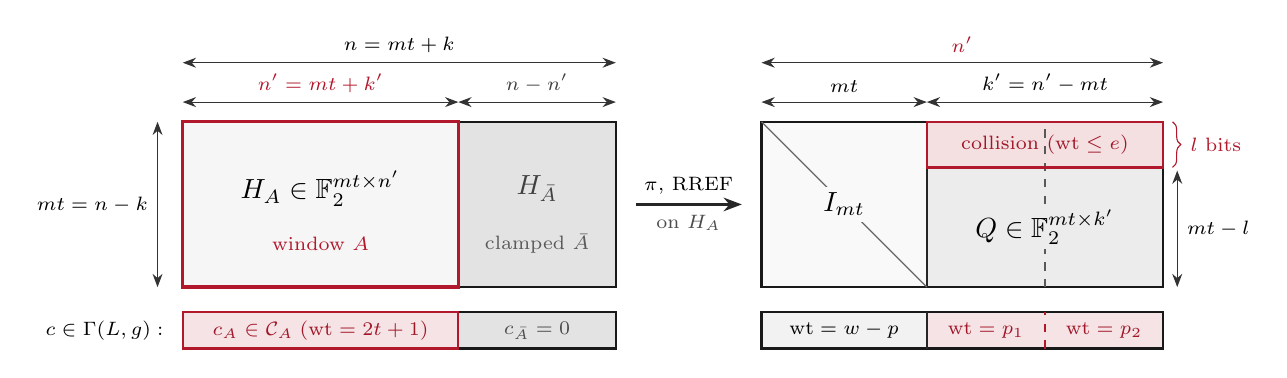
\begin{tikzpicture}[
    >=Stealth,
    font=\footnotesize,
    dimarrow/.style={<->, >=Stealth, thin, draw=black!80},
    matborder/.style={thick, draw=black!90}
]
    % === Left panel: Full H_pub partitioned into H_A and H_{\bar{A}} ===
    \fill[gray!7] (0, 0) rectangle (3.5, 2.1);
    \fill[gray!22] (3.5, 0) rectangle (5.5, 2.1);
    \draw[matborder] (0, 0) rectangle (5.5, 2.1);
    \draw[very thick, draw=accentred] (0, 0) rectangle (3.5, 2.1);

    % Dimension arrows for H_pub
    \draw[dimarrow] (-0.32, 0) -- node[left, font=\scriptsize] {$mt = n - k$} (-0.32, 2.1);
    \draw[dimarrow] (0, 2.35) -- node[above, font=\scriptsize, text=accentred] {$n' = mt + k'$} (3.5, 2.35);
    \draw[dimarrow] (3.5, 2.35) -- node[above, font=\scriptsize, text=black!75] {$n - n'$} (5.5, 2.35);
    \draw[dimarrow] (0, 2.85) -- node[above, font=\scriptsize] {$n = mt + k$} (5.5, 2.85);

    % Symbols inside H_pub
    \node[font=\normalsize] at (1.75, 1.25) {$H_A \in \F_2^{mt \times n'}$};
    \node[font=\scriptsize, text=accentred] at (1.75, 0.55) {window $A$};
    \node[font=\normalsize, text=black!75] at (4.5, 1.25) {$H_{\bar{A}}$};
    \node[font=\scriptsize, text=black!65] at (4.5, 0.55) {clamped $\bar{A}$};

    % Codeword bar below H_pub
    \fill[accentred!12] (0, -0.78) rectangle (3.5, -0.32);
    \fill[gray!22] (3.5, -0.78) rectangle (5.5, -0.32);
    \draw[matborder] (0, -0.78) rectangle (5.5, -0.32);
    \draw[thick, draw=accentred] (0, -0.78) rectangle (3.5, -0.32);
    \node[left, font=\scriptsize] at (-0.12, -0.55) {$c \in \Gamma(L, g):$};
    \node[font=\scriptsize, text=accentred!90!black] at (1.75, -0.55) {$c_A \in \mathcal{C}_A\; (\wt = 2t + 1)$};
    \node[font=\scriptsize, text=black!70] at (4.5, -0.55) {$c_{\bar{A}} = 0$};

    % === Transition arrow between panels ===
    \draw[->, >=Stealth, thick, draw=black!85] (5.75, 1.05) -- node[above, font=\scriptsize] {$\pi,\, \RREF$} node[below, font=\scriptsize, text=black!70] {on $H_A$} (7.10, 1.05);

    % === Right panel: RREF [I_{mt} | Q] on shortened window H_A ===
    \begin{scope}[xshift=7.35cm]
        \fill[gray!5] (0, 0) rectangle (2.1, 2.1);
        \fill[gray!15] (2.1, 0) rectangle (5.1, 2.1);
        % Highlighted l-bit collision window on top of Q
        \fill[accentred!14] (2.1, 1.52) rectangle (5.1, 2.1);
        \draw[matborder] (0, 0) rectangle (5.1, 2.1);
        \draw[thick, draw=black!85] (2.1, 0) -- (2.1, 2.1);
        \draw[thin, dashed, draw=black!65] (3.6, 0) -- (3.6, 2.1);
        \draw[thick, draw=accentred] (2.1, 1.52) rectangle (5.1, 2.1);
        % Diagonal of I_{mt}
        \draw[thin, draw=black!60] (0, 2.1) -- (2.1, 0);

        % Dimension arrows for \tilde{H}_A
        \draw[dimarrow] (0, 2.35) -- node[above, font=\scriptsize] {$mt$} (2.1, 2.35);
        \draw[dimarrow] (2.1, 2.35) -- node[above, font=\scriptsize] {$k' = n' - mt$} (5.1, 2.35);
        \draw[dimarrow] (0, 2.85) -- node[above, font=\scriptsize, text=accentred] {$n'$} (5.1, 2.85);
        \draw[decorate, decoration={brace, amplitude=3pt}, thin, draw=accentred] (5.22, 2.1) -- node[right=3pt, font=\scriptsize, text=accentred] {$l$ bits} (5.22, 1.52);
        \draw[dimarrow] (5.28, 0) -- node[right, font=\scriptsize] {$mt - l$} (5.28, 1.48);

        % Clean symbols inside \tilde{H}_A
        \node[font=\normalsize, fill=gray!5, inner sep=2pt] at (1.05, 1.05) {$I_{mt}$};
        \node[font=\normalsize, fill=gray!15, inner sep=1.5pt] at (3.6, 0.76) {$Q \in \F_2^{mt \times k'}$};
        \node[font=\scriptsize, text=accentred!90!black] at (3.6, 1.81) {collision ($\wt \le e$)};

        % Weight split bar below \tilde{H}_A
        \fill[gray!10] (0, -0.78) rectangle (2.1, -0.32);
        \fill[accentred!12] (2.1, -0.78) rectangle (3.6, -0.32);
        \fill[accentred!12] (3.6, -0.78) rectangle (5.1, -0.32);
        \draw[matborder] (0, -0.78) rectangle (5.1, -0.32);
        \draw[thick, draw=black!85] (2.1, -0.78) -- (2.1, -0.32);
        \draw[thin, dashed, draw=accentred] (3.6, -0.78) -- (3.6, -0.32);
        \node[font=\scriptsize] at (1.05, -0.55) {$\wt = w - p$};
        \node[font=\scriptsize, text=accentred!90!black] at (2.85, -0.55) {$\wt = p_1$};
        \node[font=\scriptsize, text=accentred!90!black] at (4.35, -0.55) {$\wt = p_2$};
    \end{scope}
\end{tikzpicture}
\caption{Matrix structure of primal shortening and multi-target $\ISD$ for a Goppa code of length $n$, codimension $mt$, and dimension $k = n - mt$. Left: permuting a full-rank $n'$-column window $A$ to the left and clamping the remaining $n - n'$ columns of $H_{\text{pub}}$ to zero restricts the search to $H_A \in \F_2^{mt \times n'}$ ($k' = n' - mt$), whose right kernel $\mathcal{C}_A = \Gamma(L_A, g)$ preserves $g(X)$. Right: each $\ISD$ round reduces $H_A \pi$ to $[I_{mt} \mid Q]$ and collides non-pivot half-lists of weights $p_1 + p_2 = p$ on an $l$-bit window to harvest codewords of odd weight $w = 2t + 1$.}
\label{fig:primal-shortening-matrix}
\end{figure}

\begin{table}[t]
\centering
\caption{Shortening windows, codeword-supply estimates, and quadratic feature compression across representative TII parameter families.}
\label{tab:shortening-windows}
{\footnotesize
\setlength{\tabcolsep}{4.0pt}
\renewcommand{\arraystretch}{1.12}
\resizebox{\textwidth}{!}{\begin{tabular}{@{}cccccccc@{}}
\toprule
\textbf{Family} & \textbf{Weight} & \textbf{Full $n$} & \textbf{Short $n'$} & \textbf{Dim $d$} & \textbf{Required} & \textbf{Available} & \textbf{Compression} \\
\midrule
$(7, 7)$   & $15$  & $112\text{--}123$ & $112$ & $62$  & $1{,}946$  & $2.79 \times 10^3$ & $1.38\times$ \\
$(8, 5)$   & $11$  & $252\text{--}253$ & $143$ & $102$ & $5{,}237$  & $7.85 \times 10^3$ & $\mathbf{4.27\times}$ ($5.3\text{k}$ vs.\ $22.4\text{k}$) \\
$(8, 6)$   & $13$  & $253\text{--}254$ & $152$ & $103$ & $5{,}348$  & $7.78 \times 10^3$ & $\mathbf{3.93\times}$ ($5.4\text{k}$ vs.\ $21.1\text{k}$) \\
$(8, 7)$   & $15$  & $221\text{--}254$ & $163$ & $106$ & $5{,}663$  & $8.32 \times 10^3$ & $\mathbf{3.42\times}$ \\
$(8, 8)$   & $17$  & $217\text{--}256$ & $175$ & $110$ & $6{,}097$  & $9.25 \times 10^3$ & $\mathbf{2.99\times}$ \\
$(8, 9)$   & $19$  & $214\text{--}255$ & $187$ & $114$ & $6{,}547$  & $9.88 \times 10^3$ & $\mathbf{2.54\times}$ (\texttt{TII-253}, $1.80\text{ s}$) \\
$(8, 10)$  & $21$  & $226\text{--}255$ & $199$ & $118$ & $7{,}013$  & $1.02 \times 10^4$ & $\mathbf{2.16\times}$ \\
$(8, 12)$  & $25$  & $223\text{--}244$ & $223$ & $126$ & $7{,}993$  & $1.03 \times 10^4$ & Solves \texttt{TII-254} in $30.4\text{ s}$ \\
$(8, 14)$  & $29$  & $246\text{--}256$ & $246$ & $133$ & $8{,}903$  & $8.49 \times 10^3$ & Illustrative window \\
$(9, 7)$   & $15$  & $482\text{--}508$ & $237$ & $173$ & $15{,}042$ & $2.20 \times 10^4$ & $\mathbf{6.56\times}$ ($15\text{k}$ vs.\ $98\text{k}$) \\
$(9, 8)$   & $17$  & $495\text{--}512$ & $253$ & $180$ & $16{,}281$ & $2.45 \times 10^4$ & $\mathbf{5.92\times}$ \\
$(9, 9)$   & $19$  & $492\text{--}509$ & $269$ & $187$ & $17{,}569$ & $2.60 \times 10^4$ & $\mathbf{5.19\times}$ \\
$(9, 10)$  & $21$  & $496\text{--}509$ & $286$ & $195$ & $19{,}101$ & $2.86 \times 10^4$ & $\mathbf{4.52\times}$ \\
$(9, 12)$  & $25$  & $493\text{--}505$ & $326$ & $217$ & $23{,}644$ & $5.23 \times 10^4$ & $\mathbf{3.31\times}$ \\
$(9, 14)$  & $29$  & $500$             & $361$ & $234$ & $27{,}486$ & $6.16 \times 10^4$ & $\mathbf{2.53\times}$ (\texttt{TII-228}) \\
$(10, 12)$ & $25$  & $1010$            & $467$ & $346$ & $60{,}021$ & $1.36 \times 10^5$ & $\mathbf{6.59\times}$ (\texttt{TII-250}, $60\text{k}$ vs.\ $396\text{k}$) \\
\midrule
$(12, 64)$ & $129$ & $3488$ (standard) & $3488$ & $2719$ & Unverified & $\approx 2^{23.47}$ & Not attacked here \\
\bottomrule
\end{tabular}}
\\[0.35em]
\parbox{\textwidth}{\footnotesize
\emph{Notes:} For each family $(m, t)$ of target weight $w = 2t + 1$, $n'$ is the shortened length, $d = n' - mt - 1$ is the affine dimension, $W_{\text{req}} = F(d) - q_{\mathrm{obs}}(m, t)$ and $W_{\text{avail}} \approx \binom{n'}{w} 2^{-mt}$ are the required and heuristic available codewords, and `Compression' is $F(n_{\max} - mt - 1) / F(d)$ across each family's `Full $n$' range.}}
\end{table}

\subsection{Cache-Resident Collision ISD vs.\ Multi-Layer BJMM}
\label{subsec:cache-isd}

\paragraph{Single-Stage Collision $\ISD$ vs.\ Multi-Layer $\BJMM$.}
For asymptotic parameters ($n = 3488, w = 129$), multi-layer representation decoders such as MMT~\cite{MMT11} and $\BJMM$~\cite{BJMM12} (and nearest-neighbor or sieving variants~\cite{MO15,DEEK24}) reduce the asymptotic exponent by splitting a weight-$p$ vector into overlapping halves across a multi-level merge tree. In the shortened TII regime ($mt \in [35, 126]$, $w \in [11, 29]$, and $k' = n' - mt \in [60, 347]$), however, single-stage collision $\ISD$ outperforms multi-layer $\BJMM$ for two concrete reasons:
\begin{enumerate}[leftmargin=2em]
    \item \textbf{Compact Half-List Combinatorics:}
    After primal shortening, each half-list has only $k'/2 \in [30, 173]$ columns, so even full triple enumeration ($p_1 = p_2 = 3$) has at most $\binom{173}{3} = 847{,}549$ entries (and $\binom{118}{3} = 266{,}916$ on \texttt{TII-228}). At $k'/2 \approx 115$, adding $\varepsilon = 1$ cancellation bits in a $3$-level $\BJMM$ tree provides minimal representation gain while introducing intermediate hash-join stages and duplicate filters that cost $5\text{--}10\times$ more instructions per candidate than a register-level 3-XOR loop.
    \item \textbf{Per-Core L1d/L2 Cache Residency vs.\ Shared DRAM Bandwidth:}
    Across $64$ physical Xeon cores (or $2{,}048\text{--}10{,}240$ physical EPYC cores on cluster runs), all cores share the socket's DRAM memory controllers. Multi-megabyte per-thread $\BJMM$ hash tables spill out of L2 ($1.25\text{ MB}$/core) and L3 cache into DRAM, stalling cores on memory bus contention. Keeping each thread's hot collision structure inside private L1d ($48\text{ KB}$) or L2 ($1.25\text{ MB}$) cache allows all cores to run at full clock speed with linear multi-core scaling.
\end{enumerate}

\paragraph{Cache-Resident Multi-Target $\ISD$ Design.}
In each round, a worker thread permutes the columns of $H_A \in \F_2^{mt \times n'}$ (with incremental pivot updates~\cite{CC98}), computes a $64$-bit word-packed RREF to obtain $\tilde{H}_A = [I_{mt} \mid Q]$ ($Q \in \F_2^{mt \times k'}$), and searches for weight-$p$ non-pivot vectors $v \in \F_2^{k'}$ whose syndrome $u = Q v \in \F_2^{mt}$ has weight $\wt(u) = w - p$. Our sampler incorporates five architectural optimizations (Table~\ref{tab:isd-modes}):

\begin{table}[t]
\centering
\caption{Multi-target $\ISD$ modes, window collision parameters, and per-thread cache footprints across TII parameter regimes.}
\label{tab:isd-modes}
{\footnotesize
\setlength{\tabcolsep}{4.0pt}
\renewcommand{\arraystretch}{1.12}
\resizebox{\textwidth}{!}{\begin{tabular}{@{}llllll@{}}
\toprule
\textbf{Mode} & \textbf{Regime} & \textbf{Parameters} & \textbf{Left Step} & \textbf{Right Step} & \textbf{Cache Footprint} \\
\midrule
Mode~3 & $mt < 88$ or $w < 21$            & $p = 3$ (no split)     & Direct triple loop      & Word-$0$ popcount prune & $\mathbf{< 8\text{ KB}}$ (L1d-resident) \\
Mode~5 & $mt \in [88, 111], w \ge 21$     & $p = 2{+}3,\, l{=}15,\, e{=}1$ & $16\times$ ball expand  & $1\times$ bucket lookup & $\mathbf{128\text{ KB}}$ bucket heads (L2) \\
Mode~6 & $mt \ge 112$, high $k'$ (\texttt{250}) & $p = 3{+}3,\, l{=}17,\, e{=}0$ & $1\times$ insert + bitmap bit & $1$-bit L1d bitmap gate & $\mathbf{16\text{ KB}}$ bitmap in \textbf{L1d} \\
Mode~7 & $mt \ge 112$, mod.\ $k'$ (\texttt{228}) & $p = 3{+}3,\, l{=}15,\, e{=}1$ & $1\times$ exact insert  & $16\times$ ball probe   & $\mathbf{128\text{ KB}}$ heads + $5.7\text{ MB}$ pool \\
\bottomrule
\end{tabular}}
\\[0.35em]
\parbox{\textwidth}{\footnotesize
\emph{Notes:} `Parameters' list the non-pivot weight split $p = p_1 + p_2$, collision window size $l$ (in bits), and allowed window Hamming weight $e$ (ball radius).}}
\end{table}

\begin{enumerate}[leftmargin=2em]
    \item \textbf{Bit-Transposed Non-Pivot Syndromes:}
    Immediately after RREF, each thread transposes the $k'$ columns of $Q$ into vertical $64$-bit words ($\lceil mt / 64 \rceil \le 2$ words per column for all $mt \le 126$), reducing column additions to $1\text{--}2$ register-level XORs and weight checks to $1\text{--}2$ hardware population-count instructions.
    \item \textbf{Mode~3: Word-$0$ Early-Pruned Lee--Brickell ($p = 3$):}
    For $mt < 88$ or $w < 21$ ($68$ of $89$ Route~A instances), enumerating non-pivot triples $(a < b < c)$ without hash tables is fastest. When $mt > 64$, the inner loop checks whether the Hamming weight of the first $64$-bit syndrome word $s_0$ already exceeds $w - 3$ before computing the second word $s_1$, pruning $>99\%$ of triples in $2$ clock cycles.
    \item \textbf{Modes~5 \& 7: Asymmetric Read/Write Ball-Collision ($l = 15, e = 1$):}
    For $mt \ge 88, w \ge 21$, we partition the $k'$ non-pivot columns into blocks of sizes $n_1$ and $n_2 = k' - n_1$ and allow ball collisions of weight $\wt(h_L \oplus h_R) \le e = 1$~\cite{BLP11} on a $15$-bit window ($2^{15} = 32{,}768$ buckets, whose $128\text{ KB}$ bucket-head array fits inside L2 cache). Because a $15$-bit ball of radius $1$ contains $1 + 15 = 16$ patterns, each RREF round captures $16\times$ more codewords than strict Stern--Dumer ($e = 0$). We flip the $16\times$ ball expansion between left insertion and right probing according to list size:
    \begin{itemize}[leftmargin=1.5em]
        \item \textbf{Mode~5 ($p = 2 + 3 = 5$, e.g., \texttt{TII-254}):}
        Setting $n_1 = \min(145, \lfloor 0.42 k' \rfloor)$, the asymmetric split makes the left pair list ($\binom{53}{2} = 1{,}378$ on \texttt{TII-254}) $47\times$ smaller than the right triple list ($\binom{74}{3} = 64{,}824$). Mode~5 expands $16\times$ on left insertion ($\le 1.67 \times 10^5$ nodes across all families), so the hot right loop performs a single lookup per triple.
        \item \textbf{Mode~7 ($p = 3 + 3 = 6$, e.g., \texttt{TII-228}):}
        With balanced halves $n_1 = \lfloor k'/2 \rfloor$, both sides enumerate triples ($\binom{118}{3} \approx 2.67 \times 10^5$), where $16\times$ left expansion would spill to DRAM. Mode~7 inserts once on the left ($5.7\text{ MB}$ pool) and probes $16$ buckets on the right, keeping the $128\text{ KB}$ bucket-head array in L2 cache.
    \end{itemize}
    \item \textbf{Mode~6: $16\text{ KB}$ L1d-Bitmap Pre-Filtered Stern--Dumer ($p = 3 + 3 = 6, l = 17$):}
    On \texttt{TII-250} ($k'=347$, $\binom{173}{3} = 847{,}549$ triples/side), Mode~6 uses a $17$-bit window ($131{,}072$ buckets, $\approx 8\text{ MB}$ per thread) guarded by a $16\text{ KB}$ occupancy bitmap ($2{,}048$ $64$-bit words) that stays 100\% resident in the $48\text{ KB}$ L1d cache. Left insertions set bit $h$ in the bitmap and record $h$ in a compact dirty-bucket list; right-side triples test bit $h$ in L1d first to reject empty buckets without touching the $8\text{ MB}$ bucket table, and only dirty buckets are reset at the end of the round.
    \item \textbf{Lock-Free Atomic Global Deduplication:}
    All threads insert discovered weight-$w$ codewords into a shared $2^{22}$-slot open-addressing hash table via $64$-bit FNV-1a support hashes and atomic compare-and-swap (CAS) operations, terminating as soon as the shared counter reaches $W_{\text{target}}$.
\end{enumerate}

\section{Quotient Reduction and Systematic Linear Lifting}
\label{sec:algebraic-lifting}

\subsection{Affine Chart and Public Polarization Quotient}
\label{subsec:quotient-tpub}

Given $W \ge W_{\text{req}}(n', m, t)$ harvested codewords $c \in \mathcal{C}_A$ of odd weight $w = 2t + 1$, three structural properties govern the quadratic evaluation system (Theorem~\ref{thm:shortened-lift}):
\begin{enumerate}[leftmargin=2em]
    \item \textbf{Odd-Weight Affine Hyperplane Parameterization ($d = k' - 1$):}
    Every harvested codeword has odd weight $w = 2t + 1$ and satisfies the linear parity constraint $\sum_{u \in A} c_u \equiv 1 \pmod 2$. In message coordinates $c = x^\top G_A$ ($x \in \F_2^{k'}$), this reads $\ell \cdot x = 1$ where $\ell = G_A \mathbf{1}_{n'}$. Interpolating quadratics directly in $x \in \F_2^{k'}$ would introduce $k'$ trivial parity-multiplied syzygies $x_i(\ell \cdot x + 1) = 0$. Parameterizing the affine hyperplane $\ell \cdot x = 1$ by $d = k' - 1$ free coordinates $y \in \F_2^d$ via
    \begin{equation}
    \label{eq:affine-chart}
        c(y) = c_0 + y^\top G_0 \qquad (y \in \F_2^d,\; d = k' - 1 = n' - mt - 1),
    \end{equation}
    where $\wt(c_0)$ is odd and every row of $G_0 \in \F_2^{d \times n'}$ has even weight, removes all $k'$ parity syzygies up front.
    \item \textbf{Rank-$\le m$ Multiplication Forms Up to Diagonal Correction:}
    Unlike dual-code quadratic-form attacks over $\F_{2^m}$ that target rank-$2$ alternating matrices~\cite{CMT23,BLT26,BLRT26}, Route~A pulls~\eqref{eq:e2-quadratic} back over $\F_2$ via linear functionals $F: \F_q \to \F_2$, giving $\sum_{u < v} c_u c_v F(z_u z_v) = F(\bar{g}_{t-1}^2)$. Because the sum ranges over strictly ordered pairs $u < v$, its symmetric coefficient matrix $M_F \in \F_2^{n' \times n'}$ has off-diagonal entries $(M_F)_{uv} = F(z_u z_v)$ ($u \neq v$) and zeros on the diagonal ($(M_F)_{uu} = 0$). By contrast, the full multiplication matrix $\widetilde{M}_F \in \F_2^{n' \times n'}$ with $(\widetilde{M}_F)_{uv} = F(z_u z_v)$ for all $u, v$ (including the diagonal $(\widetilde{M}_F)_{uu} = F(z_u^2) \eqqcolon (w_F)_u$) factors through the $m$-dimensional space $\F_q$ and has $\rk_{\F_2}(\widetilde{M}_F) \le m$. Since $\widetilde{M}_F = M_F + \diag(w_F)$, pulling back by $G_0$ yields an off-diagonal bilinear polarization matrix $B_F = G_0 M_F G_0^\top \in \F_2^{d \times d}$ such that adding $G_0 \diag(w_F) G_0^\top$ drops its rank to $\le m$:
    \[
        L_F \coloneqq B_F + G_0 \diag(w_F) G_0^\top = G_0 \widetilde{M}_F G_0^\top, \qquad \rk_{\F_2}(L_F) \le m.
    \]
    \item \textbf{Public Combinatorial Polarization $T_{\text{pub}}$:}
    Every binary vector $c \in \{0, 1\}^{n'}$ of constant weight $w = 2t + 1$ satisfies the combinatorial identity
    \begin{equation}
    \label{eq:comb-weight-id}
        \sum_{0 \le u < v < n'} c_u c_v = \binom{2t+1}{2} \equiv t \pmod 2,
    \end{equation}
    independent of $(L, g)$. Substituting $c(y) = c_0 + y^\top G_0$ into~\eqref{eq:comb-weight-id} yields a public quadratic relation with bilinear polarization matrix
    \begin{equation}
    \label{eq:t-pub-main}
        T_{\text{pub}} = G_0 (J_{n'} + I_{n'}) G_0^\top \in \F_2^{d \times d},
    \end{equation}
    where $J_{n'} + I_{n'}$ has $1$ off the diagonal and $0$ on the diagonal. Projecting out $T_{\text{pub}}$ leaves an $m$-dimensional quotient space spanned by the $m$ secret bit-slice forms $B_1, \dots, B_m$.
\end{enumerate}

\begin{theorem}[Primal Shortening Invariance, Quotient Reduction, and Support Extension]
\label{thm:shortened-lift}
Let $\Gamma(L, g) = \ker_{\F_2}(H_{\text{pub}})$ be a binary Goppa code of length $n$ and dimension $k = n - mt$, and let $A \subset \{0, \dots, n-1\}$ be a subset of $n'$ coordinate indices such that $H_A \coloneqq (H_{\text{pub}})_{:, A} \in \F_2^{mt \times n'}$ has full row rank $mt$.
\begin{enumerate}[leftmargin=2em]
    \item \textbf{Shortened Goppa Invariance~\cite{MS77,KM23}:}
    The shortened primal code $\mathcal{C}_A \coloneqq \{c_A \in \F_2^{n'} : H_A c_A^\top = 0\}$ is identically the binary Goppa code $\Gamma(L_A, g)$ of length $n'$, dimension $k' = n' - mt$, and minimum distance $\ge 2t + 1$, where $L_A = (z_j)_{j \in A}$ and $g(X)$ is the unchanged Goppa polynomial.
    \item \textbf{Odd-Weight Affine Hyperplane and Bit-Sliced Polarization:}
    Let $G_A \in \F_2^{k' \times n'}$ be a generator matrix of $\mathcal{C}_A$ and $\ell = G_A \mathbf{1}_{n'} \in \F_2^{k'}$. Parameterizing the odd-weight hyperplane $\ell \cdot x = 1$ by $x(y) = e_{i_0} + E y$ for $y \in \F_2^d$ ($d = k' - 1$, where $\ell_{i_0} = 1$ and $\operatorname{im}(E) = \ker(\ell^\top)$) and setting $G_0 = E^\top G_A \in \F_2^{d \times n'}$ and $c_0 = (G_A)_{i_0, :}$, every $\F_2$-linear functional $F \in \F_q^\vee$ pulls $e_2(z_S) = \bar{g}_{t-1}^2$ back to an affine quadratic relation $q_F(y) = 0$ on $y \in \F_2^d$ whose symmetric bilinear polarization matrix $B_F \in \F_2^{d \times d}$ ($B_{F,ii} = 0$) satisfies
    \begin{equation}
    \label{eq:bf-decomp}
        B_F = G_0\,M_F\,G_0^\top,
        \qquad
        L_F \coloneqq B_F + G_0 \diag(w_F) G_0^\top = G_0\,\widetilde{M}_F\,G_0^\top,
        \qquad
        \rk_{\F_2}(L_F) \le m,
    \end{equation}
    where $(M_F)_{uv} = F(z_u z_v)$ for $u \neq v$ with $(M_F)_{uu} = 0$, $(w_F)_u = F(z_u^2)$, and $(\widetilde{M}_F)_{uv} = F(z_u z_v)$ for all $u, v \in A$ has $\rk_{\F_2}(\widetilde{M}_F) \le m$.
    \item \textbf{Public Exceptional Direction Elimination:}
    On every weight-$(2t+1)$ codeword $c \in \mathcal{C}_A$, the identity $\sum_{u < v} c_u c_v = \binom{2t+1}{2} \equiv t \pmod 2$ induces a public quadratic relation on $y \in \F_2^d$ with polarization matrix $T_{\text{pub}} = G_0 (J_{n'} + I_{n'}) G_0^\top \in \F_2^{d \times d}$. When $T_{\text{pub}} \neq 0$, it can be quotiented out; if the $m$ secret relations are independent of each other and of $T_{\text{pub}}$, their classes span an $m$-dimensional subspace of the quotient.
    \item \textbf{Closed-Form $O(n)$ Support Extension Outside $A$~\cite{KM23}:}
    Assume $t \ge 2$ and that the recovered $(L_A, \bar{g})$ is compatible with a representation of the full public code. Choosing $mt$ independent columns $P_0 \subset A$, the unique basis change $T = H_{\text{raw}}(L_A, \bar{g})_{:, P_0} (H_A)_{:, P_0}^{-1} \in \mathrm{GL}_{mt}(\F_2)$ unscrambles the entire public key $\widetilde{H} = T H_{\text{pub}}$, and reading the first two $m$-bit field slices $v_{0, j}, v_{1, j} \in \F_q$ of each column $j \notin A$ yields~\cite{KM23,Ved26,Wei26,Saa26a,Saa26b}
    \begin{equation}
    \label{eq:support-ext}
        z_j = \frac{v_{1, j}}{v_{0, j}} \qquad (\forall\, j \in \{0, \dots, n-1\} \setminus A).
    \end{equation}
\end{enumerate}
\end{theorem}

\begin{proof}
\emph{Part~1:} A vector $c \in \F_2^n$ with $c_j = 0$ for $j \notin A$ satisfies $H_{\text{pub}} c^\top = 0 \iff H_A c_A^\top = 0$, and its Goppa syndrome $\sum_{j \in A} c_j / (X - z_j) \equiv 0 \pmod{g(X)}$ is the defining condition of $\Gamma(L_A, g)$. Since $\rk_{\F_2}(H_A) = mt$ and $g(X)$ is square-free of degree $t$, $\dim_{\F_2}\mathcal{C}_A = n' - mt = k'$ and $d_{\min}(\mathcal{C}_A) \ge 2t + 1$.

\emph{Part~2:} Expanding $c_u(y) c_v(y)$ with $c_u(y) = c_{0, u} + \sum_{a=1}^d y_a (G_0)_{au}$ inside the quadratic relation $q_F(y) = \sum_{u < v} c_u(y) c_v(y) F(z_u z_v) + F(\bar{g}_{t-1}^2) = 0$ over $\F_2$, the diagonal quadratic terms $y_a^2 = y_a$ merge into the linear part of $q_F(y)$, while for $a < b$ the coefficient of $y_a y_b$ is
\[
    (B_F)_{ab} = \sum_{u < v}\!\big((G_0)_{au}(G_0)_{bv} + (G_0)_{bu}(G_0)_{av}\big)(M_F)_{uv}
    = \sum_{u \neq v} (G_0)_{au}(M_F)_{uv}(G_0)_{bv}
    = (G_0 M_F G_0^\top)_{ab}.
\]
Because $M_F$ is symmetric with zero diagonal, $(G_0 M_F G_0^\top)_{aa} = \sum_{u < v}(G_0)_{au}(G_0)_{av}((M_F)_{uv} + (M_F)_{vu}) = 0$ over $\F_2$, so $B_F = G_0 M_F G_0^\top$ holds on all entries. Next, fix an $\F_2$-basis $e_1, \dots, e_m$ of $\F_q$ with dual coordinates $e_1^*, \dots, e_m^* \in \F_q^\vee$ so $z_u = \sum_{r=1}^m e_r^*(z_u) e_r$. By $\F_2$-linearity of $F$, $(\widetilde{M}_F)_{uv} = F(z_u z_v) = \sum_{r=1}^m e_r^*(z_u) F(e_r z_v)$ is a sum of $m$ rank-$1$ outer products over $\F_2$, so $\rk_{\F_2}(\widetilde{M}_F) \le m$ and $L_F = G_0(M_F + \diag(w_F))G_0^\top = G_0 \widetilde{M}_F G_0^\top$ has rank $\le m$.

\emph{Part~3:} Every weight-$(2t+1)$ vector has $\binom{2t+1}{2} = t(2t+1) \equiv t \pmod 2$ active pairs $u < v$. Replacing $M_F$ in Part~2 by the off-diagonal all-ones matrix $J_{n'} + I_{n'}$ yields the polarization $T_{\text{pub}} = G_0(J_{n'} + I_{n'})G_0^\top$.

\emph{Part~4:} Under compatibility, $T H_{\text{pub}} = H_{\text{raw}}(L, \bar{g})$ is uniquely determined by inverting its restriction to the $mt$ independent columns $P_0 \subset A$. Its first two $m$-bit field slices in column $j \notin A$ equal $v_{0, j} = 1/\bar{g}(z_j)$ and $v_{1, j} = z_j/\bar{g}(z_j)$, whose ratio is $z_j$. Full row-space equality $\RREF(H_{\text{raw}}(\hat{L}, \bar{g})) = H_{\text{pub}}$ is verified before accepting the extended key.
\end{proof}

\begin{proposition}[Conditional Relation-Space Identification]
\label{prop:quotient-dim}
Let $E$ evaluate the $F(d) = 1 + d + \binom{d}{2}$ Boolean affine quadratic monomials on the harvested weight-$(2t+1)$ words, and let $U$ be the span of the $m$ secret quadratic relations and the public relation. If these $m + 1$ relations are independent and $\rk_{\F_2}(E) = F(d) - (m + 1)$, then $\ker E = U$ (cf.~\cite{CMSU25} on concrete rank verification in structured algebraic code systems). Across our solved Route~A instances, the observed kernel dimension follows the profile
\begin{equation}
\label{eq:quotient-dim}
    q_{\mathrm{obs}}(m, t) =
    \begin{cases}
        2m + 1 & \text{if } t = 5, \\
        m + 1  & \text{if } t \ge 4 \text{ and } t \neq 5.
    \end{cases}
\end{equation}
For the $84$ solved Route~A instances with $t \neq 5$, quotienting $\ker E$ by $T_{\text{pub}}$ leaves an $m$-dimensional quotient space. For the $5$ solved instances with $t = 5$ (where analogous $t = 5$ degeneracies and extra kernel relations were independently observed on the shortened-dual and hold-out sides in~\cite{BLT26,Wei26}), quotienting by $T_{\text{pub}}$ leaves a $2m$-dimensional quotient; a Gray-code rank census and subspace probe isolate the true $m$-dimensional subspace in $< 0.2\text{ s}$.
\end{proposition}

\subsection{Systematic Linear Lifting and Support Extension}
\label{subsec:linear-lift}

Given $m$ basis matrices $B_1, \dots, B_m \in \F_2^{d \times d}$ representing the $m$-dimensional secret quotient space (since each row of $G_0$ has even weight, $G_0 \mathbf{1}_{n'} = 0$ and $(G_0 G_0^\top)_{aa} = 0$, so $T_{\text{pub}} = G_0 \diag(\mathbf{1}_{n'}) G_0^\top$ and representatives differing by $T_{\text{pub}}$ simply shift $w^{(r)} \mapsto w^{(r)} + \mathbf{1}_{n'}$), each $r \in \{1, \dots, m\}$ admits a binary diagonal weight vector $w^{(r)} \in \F_2^{n'}$ ($(w^{(r)})_u = F_r(z_u^2)$) such that
\begin{equation}
\label{eq:minrank-raw}
    L^{(r)} = B_r + G_0 \diag(w^{(r)}) G_0^\top \quad \text{has} \quad \rk_{\F_2}(L^{(r)}) = m.
\end{equation}

\paragraph{Decoupling Pivot Weights via Systematic Coordinates $[I_d \mid P]$.}
Whereas generic MinRank modelings such as Kipnis--Shamir~\cite{KS99} and Support-Minors~\cite{BBC20} produce bilinear systems solved via Gr\"{o}bner bases or XL, the unknowns $w^{(r)}$ here enter only through a diagonal matrix sandwiched by the known public matrix $G_0$. Since $G_0 \in \F_2^{d \times n'}$ has full row rank $d$, an invertible row transformation $U \in \mathrm{GL}_d(\F_2)$ and column permutation put $G_0$ into systematic form:
\begin{equation}
\label{eq:gs-sys}
    G_s \coloneqq U G_0 = \big[\, I_d \;\big|\; P \,\big] \in \F_2^{d \times n'},
\end{equation}
where $I_d$ is the $d \times d$ identity on the $d$ pivot columns and $P \in \F_2^{d \times (mt+1)}$ is the non-pivot block on the remaining $n' - d = mt + 1$ columns. We split $w^{(r)} = (u^{(r)}, z^{(r)})$ into $d$ pivot weights $u^{(r)} \in \F_2^d$ and $mt + 1$ non-pivot weights $z^{(r)} \in \F_2^{mt+1}$. In the transformed basis $B_r \leftarrow U B_r U^\top$, the diagonal pullback decomposes as
\[
    \big[\, I_d \;\big|\; P \,\big]
    \begin{pmatrix} \diag(u^{(r)}) & 0 \\ 0 & \diag(z^{(r)}) \end{pmatrix}
    \begin{pmatrix} I_d \\ P^\top \end{pmatrix}
    = \diag(u^{(r)}) + P \diag(z^{(r)}) P^\top.
\]
Hence the rank-$m$ target matrix $L^{(r)} \in \F_2^{d \times d}$ takes the exact structural form
\begin{equation}
\label{eq:lifted-form}
    L^{(r)} = \underbrace{B_r + P \diag(z^{(r)}) P^\top}_{\text{controls all off-diagonal entries } (i \neq j)} + \underbrace{\diag(u^{(r)})}_{\text{only on the main diagonal }(i = j)},
    \qquad \rk_{\F_2}(L^{(r)}) = m.
\end{equation}
Because all $d$ pivot unknowns $u^{(r)}$ are trapped on the main diagonal (Figure~\ref{fig:systematic-lifting-matrix}), every off-diagonal entry $(i \neq j)$ of $L^{(r)}$ depends \emph{only} on the $mt + 1$ non-pivot weights $z^{(r)}$. This enables a three-step purely $\F_2$-linear lift:

\begin{figure}[t]
\centering
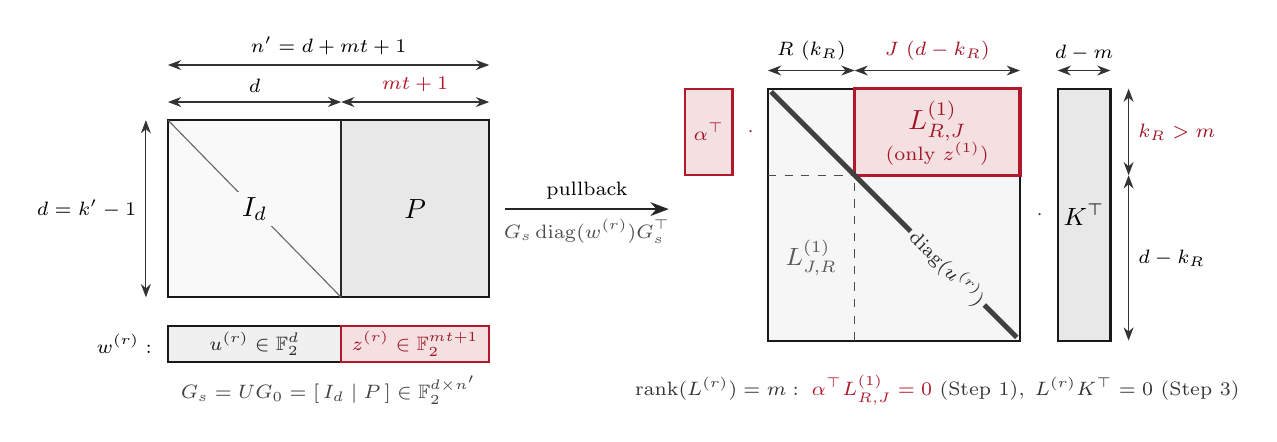
\begin{tikzpicture}[
    >=Stealth,
    font=\footnotesize,
    dimarrow/.style={<->, >=Stealth, thin, draw=black!80},
    matborder/.style={thick, draw=black!90}
]
    % === Left Panel: Systematic generator G_s = [I_d | P] and weight split w^{(r)} = (u^{(r)}, z^{(r)}) ===
    \fill[gray!5] (0, 0.30) rectangle (2.20, 2.55);
    \fill[gray!18] (2.20, 0.30) rectangle (4.08, 2.55);
    \draw[matborder] (0, 0.30) rectangle (4.08, 2.55);
    \draw[thick, draw=black!85] (2.20, 0.30) -- (2.20, 2.55);
    % Diagonal of I_d
    \draw[thin, draw=black!60] (0, 2.55) -- (2.20, 0.30);

    % Dimension arrows on G_s
    \draw[dimarrow] (-0.28, 0.30) -- node[left, font=\scriptsize] {$d = k' - 1$} (-0.28, 2.55);
    \draw[dimarrow] (0, 2.78) -- node[above, font=\scriptsize] {$d$} (2.20, 2.78);
    \draw[dimarrow] (2.20, 2.78) -- node[above, font=\scriptsize, text=accentred] {$mt + 1$} (4.08, 2.78);
    \draw[dimarrow] (0, 3.25) -- node[above, font=\scriptsize] {$n' = d + mt + 1$} (4.08, 3.25);

    % Clean symbols inside G_s
    \node[font=\normalsize, fill=gray!5, inner sep=2pt] at (1.10, 1.42) {$I_d$};
    \node[font=\normalsize] at (3.14, 1.42) {$P$};

    % Weight vector bar below G_s
    \fill[gray!12] (0, -0.52) rectangle (2.20, -0.06);
    \fill[accentred!14] (2.20, -0.52) rectangle (4.08, -0.06);
    \draw[matborder] (0, -0.52) rectangle (4.08, -0.06);
    \draw[thick, draw=accentred] (2.20, -0.52) rectangle (4.08, -0.06);
    \node[left, font=\scriptsize] at (-0.08, -0.29) {$w^{(r)}:$};
    \node[font=\scriptsize, text=black!85] at (1.10, -0.29) {$u^{(r)} \in \F_2^d$};
    \node[font=\scriptsize, text=accentred!90!black] at (3.14, -0.29) {$z^{(r)} \in \F_2^{mt+1}$};
    \node[font=\scriptsize, text=black!75] at (2.04, -0.88) {$G_s = U G_0 = [\,I_d \mid P\,] \in \F_2^{d \times n'}$};

    % === Arrow to Right Panel ===
    \draw[->, >=Stealth, thick, draw=black!85] (4.28, 1.42) -- node[above, font=\scriptsize] {pullback} node[below, font=\scriptsize, text=black!70] {$G_s \diag(w^{(r)}) G_s^\top$} (6.36, 1.42);

    % === Right Panel: Target matrix L^{(r)} \in \F_2^{d \times d} partitioned into (R, J) x (R, J) ===
    \begin{scope}[xshift=7.62cm]
        % Background of L^{(r)} (3.2 x 3.2 square)
        \fill[gray!7] (0, -0.25) rectangle (3.2, 2.95);
        % Highlight off-diagonal block L^{(1)}_{R, J} (top-right: x in [1.1, 3.2], y in [1.85, 2.95])
        \fill[accentred!14] (1.1, 1.85) rectangle (3.2, 2.95);
        % Outer border of L^{(r)}
        \draw[matborder] (0, -0.25) rectangle (3.2, 2.95);
        % Partition lines for R (size k_R) and J (size d - k_R)
        \draw[thin, dashed, draw=black!70] (1.1, -0.25) -- (1.1, 2.95);
        \draw[thin, dashed, draw=black!70] (0, 1.85) -- (3.2, 1.85);
        % Bold crimson border around off-diagonal block L^{(1)}_{R, J}
        \draw[very thick, draw=accentred] (1.1, 1.85) rectangle (3.2, 2.95);

        % Trapped main diagonal \diag(u^{(r)})
        \draw[line width=1.8pt, draw=black!75] (0.04, 2.91) -- (3.16, -0.21);
        \node[font=\scriptsize, text=black!85, fill=gray!7, inner sep=1.2pt, rotate=-45] at (2.28, 0.67) {$\diag(u^{(r)})$};

        % Clean symbols inside L^{(r)}
        \node[font=\normalsize, text=accentred!90!black] at (2.15, 2.54) {$L^{(1)}_{R, J}$};
        \node[font=\scriptsize, text=accentred!90!black] at (2.15, 2.12) {(only $z^{(1)}$)};
        \node[font=\small, text=black!65] at (0.55, 0.80) {$L^{(1)}_{J, R}$};

        % Left-kernel vector \alpha^\top multiplying L^{(1)}_{R, J} (Step 1)
        \fill[accentred!14] (-1.05, 1.85) rectangle (-0.45, 2.95);
        \draw[thick, draw=accentred] (-1.05, 1.85) rectangle (-0.45, 2.95);
        \node[font=\scriptsize, text=accentred!90!black] at (-0.75, 2.40) {$\alpha^\top$};
        \node[font=\scriptsize, text=accentred!90!black] at (-0.22, 2.40) {$\cdot$};

        % Shared right-kernel matrix K^\top multiplying L^{(r)} (Step 3)
        \node[font=\scriptsize, text=black!80] at (3.45, 1.35) {$\cdot$};
        \fill[gray!18] (3.68, -0.25) rectangle (4.35, 2.95);
        \draw[matborder] (3.68, -0.25) rectangle (4.35, 2.95);
        \node[font=\small] at (4.015, 1.35) {$K^\top$};

        % Dimension arrows on L^{(r)} and K^\top
        \draw[dimarrow] (0, 3.18) -- node[above, font=\scriptsize] {$R$ ($k_R$)} (1.1, 3.18);
        \draw[dimarrow] (1.1, 3.18) -- node[above, font=\scriptsize, text=accentred!90!black] {$J$ ($d - k_R$)} (3.2, 3.18);
        \draw[dimarrow] (3.68, 3.18) -- node[above, font=\scriptsize] {$d - m$} (4.35, 3.18);
        \draw[dimarrow] (4.58, 1.85) -- node[right, font=\scriptsize, text=accentred!90!black] {$k_R > m$} (4.58, 2.95);
        \draw[dimarrow] (4.58, -0.25) -- node[right, font=\scriptsize] {$d - k_R$} (4.58, 1.85);

        \node[font=\scriptsize, text=black!80] at (2.15, -0.88) {$\rk(L^{(r)}) = m:\; {\color{accentred}\alpha^\top L^{(1)}_{R, J} = 0}\text{ (Step 1)},\; L^{(r)} K^\top = 0\text{ (Step 3)}$};
    \end{scope}
\end{tikzpicture}
\caption{Systematic coordinate decomposition $G_s = [I_d \mid P]$ and block structure of $L^{(r)} = B_r + P\diag(z^{(r)})P^\top + \diag(u^{(r)}) \in \F_2^{d \times d}$. Trapping all $d$ pivot weights $u^{(r)} \in \F_2^d$ on the main diagonal leaves the $k_R \times (d - k_R)$ off-diagonal block $L^{(1)}_{R, J} = (B_1)_{R, J} + P_{R,:}\diag(z^{(1)})P_{J,:}^\top$ (highlighted) dependent solely on the $mt + 1$ non-pivot weights $z^{(1)}$. Step~1 recovers $z^{(1)}$ from the left kernel $\alpha^\top L^{(1)}_{R, J} = 0$; Step~2 completes $u^{(1)}$; Step~3 recovers $w^{(2)}, \dots, w^{(m)}$ against the shared right kernel $K^\top \in \F_2^{d \times (d-m)}$.}
\label{fig:systematic-lifting-matrix}
\end{figure}

\begin{enumerate}[leftmargin=2em]
    \item \textbf{Step 1: Off-Diagonal Kernel Linearization for $z^{(1)}$.}
    Partition $\{1, \dots, d\}$ into a row block $R$ of size $k_R > m$ (e.g., $k_R = 30$) and its complement $J = \{1, \dots, d\} \setminus R$ ($|J| = d - k_R$). Because $R \cap J = \emptyset$, the $k_R \times |J|$ submatrix $L^{(1)}_{R, J}$ lies entirely off the main diagonal, where $\diag(u^{(1)})$ vanishes:
    \begin{equation}
    \label{eq:off-diag-block}
        L^{(1)}_{R, J} = (B_1)_{R, J} + P_{R, :} \diag(z^{(1)}) P_{J, :}^\top \in \F_2^{k_R \times |J|}.
    \end{equation}
    When $\rk_{\F_2}(L^{(1)}_{R, J}) = m$, its left kernel has dimension $k_R - m$: any left-kernel vector $\alpha \in \F_2^{k_R}$ satisfies $\alpha^\top (B_1)_{R, J} + (\alpha^\top P_{R, :}) \diag(z^{(1)}) P_{J, :}^\top = 0$. Absorbing $z^{(1)}$ into the auxiliary vector $y = (\alpha^\top P_{R, :}) \odot z^{(1)} \in \F_2^{mt+1}$ ($y_h = (\alpha^\top P_{R, :})_h \cdot z^{(1)}_h$) produces the homogeneous linear system
    \begin{equation}
    \label{eq:z-linearized}
        \alpha^\top (B_1)_{R, J} + y^\top P_{J, :}^\top = 0
        \;\iff\;
        \big[\, (B_1)_{R, J}^\top \;\big|\; P_{J, :} \,\big] \begin{pmatrix} \alpha \\ y \end{pmatrix} = 0.
    \end{equation}
    When the $(k_R - m)$-dimensional space of true pairs $(\alpha, y)$ exhausts the kernel of $[(B_1)_{R, J}^\top \mid P_{J, :}]$, Gaussian elimination recovers $(\alpha, y)$ and reads off $z^{(1)}_h = y_h$ from any kernel vector with $(\alpha^\top P_{R, :})_h = 1$.

    \item \textbf{Step 2: Sliding Off-Diagonal Kernel for Pivot Diagonal $u^{(1)}$.}
    With $z^{(1)}$ known, $\mathrm{Off}_1 \coloneqq B_1 + P \diag(z^{(1)}) P^\top$ is known and equals $L^{(1)}$ off the diagonal. For each index $j \in \{1, \dots, d\}$, choosing $m$ rows $i_1, \dots, i_m \neq j$, setting $R = \{j, i_1, \dots, i_m\}$, and finding the $1$-dimensional left kernel $(1, \alpha_1, \dots, \alpha_m)$ of $(\mathrm{Off}_1)_{R, R^c}$ determines the diagonal entry via column $j$:
    \begin{equation}
    \label{eq:diag-complete}
        L^{(1)}_{j, j} = \sum_{s=1}^m \alpha_s (\mathrm{Off}_1)_{i_s, j},
        \qquad
        u^{(1)}_j = L^{(1)}_{j, j} + (\mathrm{Off}_1)_{j, j}.
    \end{equation}

    \item \textbf{Step 3: Shared-Kernel Multi-RHS Solve for $r = 2, \dots, m$.}
    From the completed matrix $L^{(1)}$, we compute its $(d - m) \times d$ right kernel matrix $K$ ($L^{(1)} K^\top = 0$). Because all $m$ matrices $L^{(1)}, \dots, L^{(m)}$ share the same $m$-dimensional column space, every $L^{(r)}$ ($r = 2, \dots, m$) annihilates $K^\top$:
    \begin{equation}
    \label{eq:shared-kernel-rhs}
        L^{(r)} K^\top = 0
        \;\iff\;
        \Big(G_s \diag(w^{(r)}) G_s^\top\Big) K^\top = B_r K^\top \qquad (r = 2, \dots, m).
    \end{equation}
    Because the coefficient operator $w \mapsto (G_s \diag(w) G_s^\top) K^\top$ is independent of $r$, a single matrix factorization over $\F_2$ recovers all remaining weight vectors $w^{(2)}, \dots, w^{(m)}$ simultaneously.
\end{enumerate}

\paragraph{Field Alignment, Polynomial Square Root, and $O(n)$ Support Extension.}
Choosing an invertible $m \times m$ principal block $L^{(1)}_{I, I}$ and forming $A_r = (L^{(1)}_{I, I})^{-1} L^{(r)}_{I, I}$ yields an $\F_2$-subalgebra isomorphic to $\F_{2^m}$~\cite{Saa26a,Ved26}; matching an irreducible characteristic polynomial with $f(x)$ aligns $(w^{(1)}_u, \dots, w^{(m)}_u)$ with $\F_q$ and recovers $z_u = \sqrt{z_u^2}$ for all $u \in A$. A single harvested weight-$(2t+1)$ codeword $c \in \mathcal{C}_A$ then gives $\bar{g}(X) = \sqrt{\sigma'_S(X)}$ by Theorem~\ref{thm:deriv-square}, and Theorem~\ref{thm:shortened-lift}(4) extends $L_A$ to all $n - n'$ remaining columns via $z_j = v_{1, j} / v_{0, j}$~\cite{KM23} in $O(n)$ field divisions.

\subsection{End-to-End Walkthrough on \texorpdfstring{\texttt{TII-253}}{TII-253}}
\label{subsec:walkthrough-253}

We now trace the complete Route~A pipeline from an algebraic and matrix perspective in terms of the Goppa parameters $(n, m, t, k = n - mt)$ and shortened parameters $(n', k' = n' - mt, d = k' - 1)$. We illustrate every stage on \texttt{TII-253} ($(n, m, t, k) = (214, 8, 9, 142)$, codimension $mt = 72$, minimum odd weight $w = 2t + 1 = 19$). As shown in Figure~\ref{fig:walkthrough-pipeline}(a), rather than solving for the secret support directly in the ambient spaces along the bottom row, Route~A follows a zigzag path (in red) through shortened and quotient spaces along the top row before lifting back to the full private key $(L, \bar{g})$.

\begin{figure}[t]
\centering
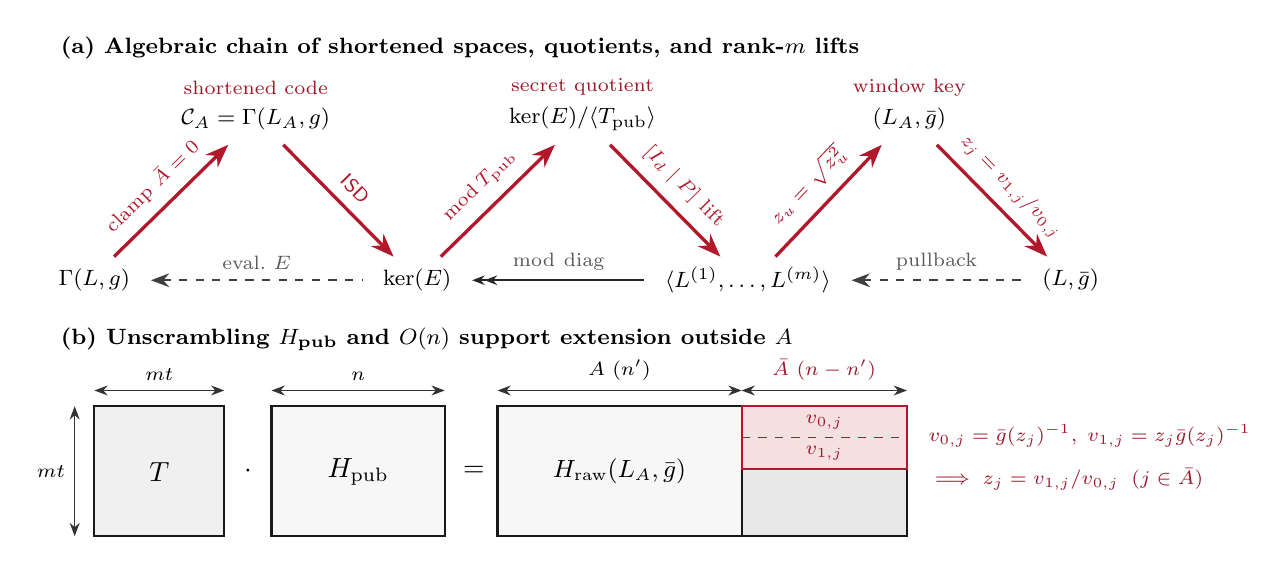
\begin{tikzpicture}[
    >=Stealth,
    font=\footnotesize,
    dimarrow/.style={<->, >=Stealth, thin, draw=black!80},
    matborder/.style={thick, draw=black!90},
    projarrow/.style={-{Stealth[length=4.5pt]Stealth[length=4.5pt]}, thick, draw=black!85},
    algpath/.style={->, >=Stealth, very thick, draw=accentred}
]
    % =========================================================================
    % PART (a): Algebraic Chain & Zigzag Trajectory
    % =========================================================================
    \node[anchor=west, font=\footnotesize\bfseries] at (-0.55, 2.95) {(a) Algebraic chain of shortened spaces, quotients, and rank-$m$ lifts};

    % Bottom row: 4 Ambient / Lifted Spaces (y = 0.0, x = 0.0, 4.1, 8.3, 12.4)
    \node (B0) at (0.0, 0.0) {$\Gamma(L, g)$};
    \node (B1) at (4.1, 0.0) {$\ker(E)$};
    \node (B2) at (8.3, 0.0) {$\langle L^{(1)}, \dots, L^{(m)} \rangle$};
    \node (B3) at (12.4, 0.0) {$(L, \bar{g})$};

    % Top row: 3 Interleaved Shortened / Quotient Spaces (y = 2.05, x = 2.05, 6.2, 10.35)
    \node (T1) at (2.05, 2.05) {$\mathcal{C}_A = \Gamma(L_A, g)$};
    \node[font=\scriptsize, text=accentred!90!black] at (2.05, 2.45) {shortened code};

    \node (T2) at (6.2, 2.05) {$\ker(E) / \langle T_{\text{pub}} \rangle$};
    \node[font=\scriptsize, text=accentred!90!black] at (6.2, 2.45) {secret quotient};

    \node (T3) at (10.35, 2.05) {$(L_A, \bar{g})$};
    \node[font=\scriptsize, text=accentred!90!black] at (10.35, 2.45) {window key};

    % Structural black arrows along bottom row
    \draw[<-, >=Stealth, thick, draw=black!75, dashed, shorten <=4pt, shorten >=4pt] (B0.east) -- node[above, font=\scriptsize, text=black!65] {eval.\ $E$} (B1.west);
    \draw[projarrow, shorten <=4pt, shorten >=4pt] (B2.west) -- node[above, font=\scriptsize, text=black!65] {$\bmod\,\diag$} (B1.east);
    \draw[<-, >=Stealth, thick, draw=black!75, dashed, shorten <=4pt, shorten >=4pt] (B2.east) -- node[above, font=\scriptsize, text=black!65] {pullback} (B3.west);

    % Algorithmic Zigzag Path in Crimson (6 strictly disjoint diagonal segments)
    \draw[algpath] (0.25, 0.30) -- node[pos=0.48, sloped, above=1pt, font=\scriptsize, text=accentred] {clamp $\bar{A}=0$} (1.70, 1.72);
    \draw[algpath] (2.40, 1.72) -- node[pos=0.52, sloped, above=1pt, font=\scriptsize, text=accentred] {$\ISD$} (3.80, 0.30);
    \draw[algpath] (4.40, 0.30) -- node[pos=0.48, sloped, above=1pt, font=\scriptsize, text=accentred] {$\bmod\, T_{\text{pub}}$} (5.85, 1.72);
    \draw[algpath] (6.55, 1.72) -- node[pos=0.52, sloped, above=1pt, font=\scriptsize, text=accentred] {$[I_d \mid P]$ lift} (7.95, 0.30);
    \draw[algpath] (8.65, 0.30) -- node[pos=0.48, sloped, above=1pt, font=\scriptsize, text=accentred] {$z_u = \sqrt{z_u^2}$} (10.00, 1.72);
    \draw[algpath] (10.70, 1.72) -- node[pos=0.52, sloped, above=1pt, font=\scriptsize, text=accentred] {$z_j = v_{1,j}/v_{0,j}$} (12.10, 0.30);

    % =========================================================================
    % PART (b): Matrix Structure of O(n) Support Extension
    % =========================================================================
    \node[anchor=west, font=\footnotesize\bfseries] at (-0.55, -0.75) {(b) Unscrambling $H_{\text{pub}}$ and $O(n)$ support extension outside $A$};

    \begin{scope}[yshift=-3.45cm]
        % Left: T * H_{pub}
        \fill[gray!12] (0.0, 0.20) rectangle (1.65, 1.85);
        \draw[matborder] (0.0, 0.20) rectangle (1.65, 1.85);
        \draw[dimarrow] (-0.25, 0.20) -- node[left, font=\scriptsize] {$mt$} (-0.25, 1.85);
        \draw[dimarrow] (0.0, 2.05) -- node[above, font=\scriptsize] {$mt$} (1.65, 2.05);
        \node[font=\normalsize] at (0.825, 1.02) {$T$};

        \node[font=\normalsize] at (1.95, 1.02) {$\cdot$};

        \fill[gray!6] (2.25, 0.20) rectangle (4.45, 1.85);
        \draw[matborder] (2.25, 0.20) rectangle (4.45, 1.85);
        \draw[dimarrow] (2.25, 2.05) -- node[above, font=\scriptsize] {$n$} (4.45, 2.05);
        \node[font=\normalsize] at (3.35, 1.02) {$H_{\text{pub}}$};

        \node[font=\normalsize] at (4.82, 1.02) {$=$};

        % Right: Unscrambled \widetilde{H} = H_{raw}(L, \bar{g}) partitioned into A and \bar{A}
        \begin{scope}[xshift=5.12cm]
            \fill[gray!6] (0, 0.20) rectangle (3.1, 1.85);
            \fill[gray!18] (3.1, 0.20) rectangle (5.2, 1.85);
            % Highlight top two m-bit field-slice rows in \bar{A}
            \fill[accentred!14] (3.1, 1.05) rectangle (5.2, 1.85);

            \draw[matborder] (0, 0.20) rectangle (5.2, 1.85);
            \draw[thick, draw=black!90] (3.1, 0.20) -- (3.1, 1.85);
            \draw[thin, dashed, draw=accentred] (3.1, 1.45) -- (5.2, 1.45);
            \draw[thick, draw=accentred] (3.1, 1.05) rectangle (5.2, 1.85);

            % Dimension arrows
            \draw[dimarrow] (0, 2.05) -- node[above, font=\scriptsize] {$A$ ($n'$)} (3.1, 2.05);
            \draw[dimarrow] (3.1, 2.05) -- node[above, font=\scriptsize, text=accentred!90!black] {$\bar{A}$ ($n - n'$)} (5.2, 2.05);

            % Clean symbols inside \widetilde{H}
            \node[font=\small] at (1.55, 1.02) {$H_{\text{raw}}(L_A, \bar{g})$};
            \node[font=\scriptsize, text=accentred!90!black] at (4.15, 1.65) {$v_{0, j}$};
            \node[font=\scriptsize, text=accentred!90!black] at (4.15, 1.25) {$v_{1, j}$};

            % Concise callouts on right for top two m-bit field slices
            \node[right, font=\scriptsize, text=accentred!90!black] at (5.35, 1.48) {$v_{0, j} = \bar{g}(z_j)^{-1},\; v_{1, j} = z_j \bar{g}(z_j)^{-1}$};
            \node[right, font=\scriptsize\bfseries, text=accentred!90!black] at (5.35, 0.92) {$\implies z_j = v_{1, j} / v_{0, j}\;\; (j \in \bar{A})$};
        \end{scope}
    \end{scope}
\end{tikzpicture}
\caption{Algebraic and matrix overview of Route~A for a binary Goppa code of parameters $(n, m, t, k = n - mt)$. (a)~Horizontal black arrows indicate structural evaluation, diagonal-quotient, and pullback maps along the bottom row, while the solid red zigzag path traces the algorithmic steps through the shortened and quotient spaces on the top row. (b)~Once $(L_A, \bar{g})$ is known on the $n'$-column window $A$, matching $H_{\text{raw}}(L_A, \bar{g})$ on $A$ determines $T \in \mathrm{GL}_{mt}(\F_2)$ and unscrambles $T H_{\text{pub}}$ so that the top two $m$-bit field slices of every column $j \in \bar{A}$ yield $z_j = v_{1, j} / v_{0, j}$.}
\label{fig:walkthrough-pipeline}
\end{figure}

\paragraph{1. Primal Shortening and Multi-Target $\ISD$ ($H_{\text{pub}} \to \mathcal{C}_A$).}
Given the public parity-check matrix $H_{\text{pub}} \in \F_2^{mt \times n}$ of a Goppa code $\Gamma(L, g)$ with codimension $mt = n - k$, interpolating the quadratic identity $\sum_{u < v} c_u c_v F(z_u z_v) = F(\bar{g}_{t-1}^2)$ directly over the full code of dimension $k$ would require $F(k - 1) = \Theta(k^2)$ monomials and $O(k^6)$ dense linear algebra. Instead, we partition the $n$ columns into an active window $A$ of width $n' = mt + k'$ and a clamped complement $\bar{A}$ of width $n - n'$ (Figure~\ref{fig:primal-shortening-matrix}, left). Clamping $c_{\bar{A}} = 0$ projects the search onto the shortened code $\mathcal{C}_A = \ker(H_A) = \Gamma(L_A, g) \subset \F_2^{n'}$ of dimension $k' = n' - mt \ll k$, preserving $g(X)$ while leaving the per-check $\ISD$ yield $\binom{mt}{w-p} 2^{-mt}$ unchanged by Proposition~\ref{prop:isd-cancellation}. In each $\ISD$ round, reducing $H_A \pi$ to $[I_{mt} \mid Q]$ ($Q \in \F_2^{mt \times k'}$, Figure~\ref{fig:primal-shortening-matrix}, right) collides non-pivot vectors of weight $p = p_1 + p_2$ against pivot syndromes of weight $w - p$ to harvest $W \ge W_{\text{req}}(n', m, t)$ codewords of minimum odd weight $w = 2t + 1$.
\emph{On \texttt{TII-253} $(n = 214, m = 8, t = 9, mt = 72, k = 142, w = 19)$:} shortening to $n' = 187$ ($n - n' = 27$ clamped columns) reduces the code dimension from $k = 142$ to $k' = 115$ ($d = k' - 1 = 114$), compressing the quadratic monomial count by $\mathbf{1.53\times}$ from $F(141) = 10{,}012$ to $F(114) = \mathbf{6{,}556}$ (and up to $2.54\times$ across the $(8, 9)$ family at $n = 255$), and Mode~3 $\ISD$ ($p = 3$ on $Q \in \F_2^{72 \times 115}$) harvests $W = 6{,}643 \ge W_{\text{req}} = 6{,}547$ weight-$19$ codewords across $64$ physical Xeon cores in $\mathbf{0.43\text{ s}}$.

\paragraph{2. Affine Hyperplane and Public Polarization Quotient ($\mathcal{C}_A \to \langle B_1, \dots, B_m \rangle$).}
Because every harvested codeword has odd weight $w = 2t + 1$, it lies on the affine hyperplane $\ell \cdot x = 1$ in $\F_2^{k'}$, parameterized by $d = k' - 1 = n' - mt - 1$ coordinates $y \in \F_2^d$ via $c(y) = c_0 + y^\top G_0$ ($G_0 \in \F_2^{d \times n'}$, Figure~\ref{fig:walkthrough-pipeline}(a)). Evaluating the $F(d) = 1 + d + \binom{d}{2}$ quadratic monomials in $y$ across $W$ harvested codewords produces the evaluation matrix $E \in \F_2^{W \times F(d)}$. By Theorem~\ref{thm:shortened-lift}, when $t \neq 5$ the right kernel $\ker(E)$ has dimension $m + 1$, spanned by the $m$ secret bit-slice relations and the public combinatorial relation $\sum_{u < v} c_u c_v = \binom{2t+1}{2} \equiv t \pmod 2$. Quotienting $\ker(E)$ by its public polarization $T_{\text{pub}} = G_0(J_{n'} + I_{n'})G_0^\top$ isolates an $m$-dimensional space of symmetric off-diagonal bilinear forms $\langle B_1, \dots, B_m \rangle \subset \F_2^{d \times d}$.
\emph{On \texttt{TII-253}:} eliminating $E \in \F_2^{6643 \times 6556}$ yields an $(m + 1) = 9$-dimensional kernel, and quotienting out $T_{\text{pub}} \in \F_2^{114 \times 114}$ leaves $m = 8$ basis matrices $B_1, \dots, B_8 \in \F_2^{114 \times 114}$.

\paragraph{3. Systematic Coordinates and Off-Diagonal Linear Lift ($\langle B_r \rangle \to L_A$).}
Each basis matrix $B_r$ differs from a rank-$m$ multiplication pullback $L^{(r)} = G_0 \widetilde{M}_{F_r} G_0^\top$ by an unknown diagonal correction $G_0 \diag(w^{(r)}) G_0^\top$, where $(w^{(r)})_u = F_r(z_u^2)$ ($u \in A$). Transforming $G_0 \in \F_2^{d \times n'}$ into systematic form $G_s = U G_0 = [I_d \mid P]$ ($P \in \F_2^{d \times (mt+1)}$, Figure~\ref{fig:systematic-lifting-matrix}, left) partitions $w^{(r)} = (u^{(r)}, z^{(r)})$ into $d$ pivot weights $u^{(r)} \in \F_2^d$ and $mt + 1$ non-pivot weights $z^{(r)} \in \F_2^{mt+1}$, yielding
\[
    L^{(r)} = B_r + P\diag(z^{(r)})P^\top + \diag(u^{(r)}) \in \F_2^{d \times d}, \qquad \rk_{\F_2}(L^{(r)}) = m.
\]
As depicted in Figure~\ref{fig:systematic-lifting-matrix} (right), $\diag(u^{(r)})$ is trapped on the main diagonal, so for any partition $\{1, \dots, d\} = R \sqcup J$ with $|R| = k_R > m$ and $|J| = d - k_R$, the $k_R \times (d - k_R)$ off-diagonal block $L^{(1)}_{R, J} = (B_1)_{R, J} + P_{R,:}\diag(z^{(1)})P_{J,:}^\top$ depends solely on $z^{(1)}$. Its $(k_R - m)$-dimensional left kernel $\alpha^\top L^{(1)}_{R, J} = 0$ linearizes into $[(B_1)_{R, J}^\top \mid P_{J,:}](\alpha; y) = 0$ (Step~1, recovering $z^{(1)}$), after which sliding $(m+1)$-row off-diagonal kernels determine $u^{(1)}$ (Step~2) and the $(d - m)$-dimensional right kernel $K^\top$ of $L^{(1)}$ solves $L^{(r)}K^\top = 0$ for all $r = 2, \dots, m$ simultaneously (Step~3). Aligning the $m \times m$ commuting algebra with $\F_q = \F_2[x]/(f(x))$ and taking square roots recovers $z_u = \sqrt{z_u^2}$ for all $u \in A$.
\emph{On \texttt{TII-253}:} with $G_s = [I_{114} \mid P]$ ($P \in \F_2^{114 \times 73}$) and $k_R = 30$, Step~1 solves the $30 \times 84$ off-diagonal block $L^{(1)}_{R, J}$ to recover the $mt + 1 = 73$ non-pivot weights $z^{(1)} \in \F_2^{73}$, Step~2 recovers the $d = 114$ pivot weights $u^{(1)} \in \F_2^{114}$, and Step~3 solves against $K^\top \in \F_2^{114 \times 106}$ to recover $w^{(2)}, \dots, w^{(8)} \in \F_2^{187}$ and hence $L_A \in \F_{2^8}^{187}$.

\paragraph{4. Locator Square Root and Unscrambled Support Extension ($L_A \to (L, \bar{g})$).}
From a single harvested codeword $c \in \mathcal{C}_A$ with support $S \subset A$ ($|S| = 2t + 1$), Theorem~\ref{thm:deriv-square} recovers the monic Goppa polynomial $\bar{g}(X) = \sqrt{\sigma'_S(X)}$ in $\F_q[X]$. Finally, choosing an invertible $mt$-column block $P_0 \subset A$ and computing $T = H_{\text{raw}}(L_A, \bar{g})_{:, P_0} (H_A)_{:, P_0}^{-1} \in \mathrm{GL}_{mt}(\F_2)$ unscrambles the full public parity-check matrix $\widetilde{H} = T H_{\text{pub}} = H_{\text{raw}}(L, \bar{g}) \in \F_2^{mt \times n}$ (Figure~\ref{fig:walkthrough-pipeline}(b)). Reading the first two $m$-bit field slices $v_{0, j} = 1/\bar{g}(z_j)$ and $v_{1, j} = z_j/\bar{g}(z_j)$ of each external column $j \in \bar{A}$ immediately recovers the remaining $n - n'$ support elements via $z_j = v_{1, j} / v_{0, j}$~\cite{KM23}.
\emph{On \texttt{TII-253}:} inverting a $72 \times 72$ block $P_0 \subset A$ unscrambles $\widetilde{H} \in \F_2^{72 \times 214}$, and $n - n' = 27$ field divisions in $\F_{2^8}$ recover the remaining $27$ support coordinates, completing algebraic recovery and RREF verification in $\mathbf{1.37\text{ s}}$ ($\mathbf{1.80\text{ s}}$ total wall time, $0.032\text{ ch}$, $242\text{ MB}$ RAM).

\subsection{Complementary Route B on High-Rate Instances}
\label{subsec:route-b-summary}

For the single high-rate parameter family $m = 10, t = 11, mt = 110, n \in [1008, 1020]$ ($k \in [898, 910]$, rate $R \approx 0.891 > 1 - 2/t$), primal shortening in Route~A would require a window $n' \approx 443$ ($w = 23$). Instead, the dual code admits a clean degree-$3$ ($p_{\HOV} = 3$) higher-order vanishing ($\HOV$) kernel at dual shortening $s^* = 36$ ($\kappa = mt - s^* = 74, \rho = m p_{\HOV}^2 = 90$)~\cite{HW26,Hem26,Saa26a}. For these five challenges (\texttt{TII-172, 187, 240, 246, 252}), we deploy an optimized $\HOVER$ engine (Route~B; Appendix~\ref{app:route-b}): combining Frobenius rank invariance~\cite{Saa26a} with the known span dimension $\rho = 90$ replaces the $10$-matrix catalecticant rank sum over $\F_{2^{10}}$ by a single rank check $\rk\Cat(h_0) = 9$, incremental commutator intersection stabilizes the algebra $E_\beta$ from $1\text{--}2$ right-kernel blocks instead of all $650$ blocks, and Segre--Veronese fiber extraction on $450$ truncated coordinates is completed via closed-form support extension~\eqref{eq:support-ext}. Route~B solves all five $(10, 11)$ instances in $89.10\text{--}90.10\text{ s}$ on $1$ physical CPU core ($0.025\text{ ch}$), achieving two first-blood recoveries (\texttt{TII-172, 187}) and a $4.17\times$ wall-time / $50.0\times$ core-hour speedup over the $12$-core reference $\HOVER$ solver on \texttt{TII-252}~\cite{Saa26a}.

\section{Feasibility Boundary and Experimental Verification}
\label{sec:experiments}

\subsection{Parameter Regimes and the Classic McEliece Boundary}
Across the $170$ official Track-2 challenges with $\lambda_{\text{TII}} \ge 83$, the word-supply model in Proposition~\ref{prop:isd-cancellation} partitions the catalog into three regimes:
\begin{enumerate}[leftmargin=2em]
    \item \textbf{Solved Regime ($94$ Instances: $89$ via Route~A, $5$ via Route~B):}
    Whenever $n \ge n'_{\min}(m, t)$ and $mt \le 126$, the code supplies enough weight-$(2t+1)$ codewords to determine the $F(d)$ quadratic features, and our framework recovers the private key $(L, g)$.
    \item \textbf{Information-Theoretically Underdetermined Regime ($60$ Challenges with $n < n'_{\min}$):}
    In $60$ challenges with short lengths $n$ relative to $mt$ (e.g., \texttt{TII-201} with $m = 8, t = 20, n = 253, k = 93$, where $W_{\text{req}} = 4{,}270$ evaluation rows are required on $d = 92$ coordinates but the full code has only $\binom{253}{41} 2^{-160} \approx 0.224$ expected weight-$41$ codewords), the full code does not contain enough minimum-weight codewords to determine the quadratic system regardless of available compute.
    \item \textbf{Compute-Limited Regime ($16$ Challenges with $mt \in [120, 189]$) and Classic McEliece:}
    In the remaining $16$ challenges with $n \ge n'_{\min}$ and large $mt \in [120, 189]$ ($w \in [25, 43]$), the codeword supply exists in principle, but the per-iteration $\ISD$ yield~\eqref{eq:yield-cancellation} scales as $\binom{k'}{p}\binom{mt}{w-p} 2^{-mt}$, requiring $10^4\text{--}10^8+$ core-hours. For Classic McEliece standard parameters ($m \in \{12, 13\}$, $t \ge 64$, $mt \ge 768$, $w \ge 129$, $n \in [3488, 8192]$), Route~A is doubly infeasible: for \texttt{mceliece348864} ($m = 12, t = 64, mt = 768, w = 129$) at the algebraic threshold $n'_{\min} = 793$, the expected count of weight-$129$ codewords is $\binom{793}{129} 2^{-768} < 2^{-264}$ (and $< 2^{-20}$ even at full length $n$ for all $m = 13$ Classic McEliece parameter sets), while at full length $n = 3488$ ($\log_2\binom{3488}{129} - 768 \approx 23.47$), multi-target $\ISD$ for a weight-$129$ codeword exceeds $2^{240}$ operations~\cite{CC98,BJMM12} (and even single-target weight-$64$ syndrome decoding requires $2^{150.6}$ bit operations in \texttt{CryptAttackTester}~\cite{BC24}).
\end{enumerate}

\subsection{Verification and Compute Accounting on 94 Challenges}
We evaluated Route~A and Route~B across the official TII McEliece Track-2 catalog and verified all $94$ recovered keys:
\begin{itemize}[leftmargin=1.5em]
    \item \textbf{Official SageMath Verification ($94/94$ Verified):}
    Every recovered key is formatted in TII's official two-line $(g, L)$ representation and passes a complete rerun of TII's official SageMath verification script under SageMath~10.9 against the official public-key files ($94/94$ verified), with monic $\F_q$-irreducible $g(X)$ of degree $t$ across all $94$ keys.
    \item \textbf{Physical Core-Hour Accounting:}
    We count allocated physical CPU cores (excluding hyperthreads) multiplied by end-to-end wall-clock runtime across both $\ISD$ sampling and algebraic lifting. Under this metric, the $92$ single-node challenges consume $177.82$ physical core-hours combined ($87$ via Route~A on a $64$-physical-core Dual Intel Xeon Gold 6338 server, and $5$ via Route~B on $1$ physical core), while the two pure-CPU cluster challenges \texttt{TII-228} $(500, 9, 14, mt=126)$ and \texttt{TII-250} $(1010, 10, 12, mt=120)$ consume $2{,}463.3$ and $66{,}722.1$ physical core-hours ($57.1\text{ min}$ and $9.20\text{ h}$ wall time). Table~\ref{tab:campaign-regimes} summarizes all $94$ solved challenges by parameter family.
\end{itemize}

\begin{table}[t]
\centering
\caption{Summary of all $94$ solved TII Track-2 key-recovery challenges grouped by Goppa parameter family $(m, t)$.}
\label{tab:campaign-regimes}
{\footnotesize
\setlength{\tabcolsep}{3.0pt}
\renewcommand{\arraystretch}{1.02}
\resizebox{\textwidth}{!}{\begin{tabular}{@{}cccccccc>{\raggedright\arraybackslash}p{3.45cm}@{}}
\toprule
\textbf{Family} & \textbf{Route} & \textbf{Solved} & \textbf{Window} & \textbf{Med.\ Time} & \textbf{Med.\ Compute} & \textbf{Total Compute} & \textbf{RAM} & \textbf{Challenge IDs} \\
\midrule
$(7, 5)$   & A ($35$)  & $3$ ($0$)   & $n'=120\text{--}122$ & $10.9\text{ s}$ & $0.194\text{ ch}$ & $3.72\text{ ch}$     & $237\text{ MB}$ & \texttt{86, 90, 94} \\
$(7, 7)$   & A ($49$)  & $6$ ($6$)   & $n'=112$             & $0.39\text{ s}$ & $0.007\text{ ch}$ & $0.04\text{ ch}$     & $231\text{ MB}$ & \texttt{95, 103, 107, 111, 127, 133} \\
$(7, 8)$   & A ($56$)  & $4$ ($4$)   & $n'=120\text{--}124$ & $3.53\text{ s}$ & $0.063\text{ ch}$ & $0.24\text{ ch}$     & $233\text{ MB}$ & \texttt{87, 97, 102, 114} \\
$(7, 9)$   & A ($63$)  & $1$ ($1$)   & $n'=127$             & $1.76\text{ s}$ & $0.031\text{ ch}$ & $0.03\text{ ch}$     & $228\text{ MB}$ & \texttt{88} \\
$(8, 5)$   & A ($40$)  & $2$ ($0$)   & $n'=143$             & $1.53\text{ s}$ & $0.027\text{ ch}$ & $0.05\text{ ch}$     & $286\text{ MB}$ & \texttt{83, 89} \\
$(8, 6)$   & A ($48$)  & $2$ ($0$)   & $n'=152$             & $0.96\text{ s}$ & $0.017\text{ ch}$ & $0.03\text{ ch}$     & $340\text{ MB}$ & \texttt{84, 91} \\
$(8, 7)$   & A ($56$)  & $7$ ($0$)   & $n'=163$             & $1.06\text{ s}$ & $0.019\text{ ch}$ & $0.12\text{ ch}$     & $340\text{ MB}$ & \texttt{92, 110, 160, 171, 178, 212, 220} \\
$(8, 8)$   & A ($64$)  & $10$ ($7$)  & $n'=175$             & $1.32\text{ s}$ & $0.023\text{ ch}$ & $0.24\text{ ch}$     & $340\text{ MB}$ & \texttt{85, 93, 100, 112, 118, 123, 179, 186, 233, 238} \\
$(8, 9)$   & A ($72$)  & $7$ ($6$)   & $n'=187$             & $1.38\text{ s}$ & $0.024\text{ ch}$ & $0.18\text{ ch}$     & $252\text{ MB}$ & \texttt{101, 120, 126, 146, 216, 222, 253} \\
$(8, 10)$  & A ($80$)  & $10$ ($10$) & $n'=199$             & $2.02\text{ s}$ & $0.036\text{ ch}$ & $0.36\text{ ch}$     & $255\text{ MB}$ & \texttt{109, 122, 128, 139, 144, 149, 221, 224, 227, 230} \\
$(8, 11)$  & A ($88$)  & $4$ ($4$)   & $n'=212$             & $3.75\text{ s}$ & $0.067\text{ ch}$ & $0.29\text{ ch}$     & $259\text{ MB}$ & \texttt{130, 152, 157, 206} \\
$(8, 12)$  & A ($96$)  & $3$ ($2$)   & $n'=223\text{--}224$ & $28.8\text{ s}$ & $0.511\text{ ch}$ & $1.22\text{ ch}$     & $313\text{ MB}$ & \texttt{183, 203, 254} \\
$(8, 13)$  & A ($104$) & $1$ ($1$)   & $n'=233$             & $332\text{ s}$  & $5.90\text{ ch}$  & $5.90\text{ ch}$     & $254\text{ MB}$ & \texttt{232} \\
$(8, 14)$  & A ($112$) & $3$ ($3$)   & $n'=246\text{--}250$ & $82.7\text{ s}$ & $1.47\text{ ch}$  & $10.77\text{ ch}$    & $263\text{ MB}$ & \texttt{132, 165, 190} \\
$(9, 7)$   & A ($63$)  & $6$ ($0$)   & $n'=237$             & $5.50\text{ s}$ & $0.098\text{ ch}$ & $0.60\text{ ch}$     & $340\text{ MB}$ & \texttt{119, 125, 166, 210, 244, 248} \\
$(9, 8)$   & A ($72$)  & $6$ ($0$)   & $n'=253$             & $11.4\text{ s}$ & $0.203\text{ ch}$ & $1.21\text{ ch}$     & $340\text{ MB}$ & \texttt{96, 105, 113, 134, 164, 200} \\
$(9, 9)$   & A ($81$)  & $4$ ($0$)   & $n'=269$             & $39.8\text{ s}$ & $0.708\text{ ch}$ & $2.85\text{ ch}$     & $339\text{ MB}$ & \texttt{129, 189, 209, 223} \\
$(9, 10)$  & A ($90$)  & $4$ ($3$)   & $n'=286$             & $113\text{ s}$  & $2.02\text{ ch}$  & $8.73\text{ ch}$     & $351\text{ MB}$ & \texttt{138, 158, 208, 213} \\
$(9, 11)$  & A ($99$)  & $1$ ($1$)   & $n'=303$             & $408\text{ s}$  & $7.25\text{ ch}$  & $7.25\text{ ch}$     & $373\text{ MB}$ & \texttt{147} \\
$(9, 12)$  & A ($108$) & $3$ ($3$)   & $n'=326$             & $2509\text{ s}$ & $44.61\text{ ch}$ & $133.84\text{ ch}$   & $427\text{ MB}$ & \texttt{182, 188, 245} \\
$(9, 14)$  & A ($126$) & $1$ ($1$)   & $n'=361$             & $57.1\text{ min}$ & $2{,}463\text{ ch}$ & $2{,}463\text{ ch}$ & $468\text{ MB}$ & \texttt{228} \\
$(10, 11)$ & B ($110$) & $5$ ($2$)   & $s^*=36, \kappa=74$  & $89.9\text{ s}$ & $0.025\text{ ch}$ & $0.12\text{ ch}$     & $1.49\text{ GB}$ & \texttt{172, 187, 240, 246, 252} \\
$(10, 12)$ & A ($120$) & $1$ ($1$)   & $n'=467$             & $9.20\text{ h}$ & $66{,}722\text{ ch}$ & $66{,}722\text{ ch}$ & $1.28\text{ GB}$ & \texttt{250} \\
\midrule
\textbf{Total} & \textbf{A+B} & $\mathbf{94}$ ($\mathbf{55}$) & --- & --- & --- & $\mathbf{69{,}363.3\text{ ch}}$ & --- & \textbf{$92$ single-node: $177.82\text{ ch}$} \\
\bottomrule
\end{tabular}}
\\[0.35em]
\parbox{\textwidth}{\footnotesize
\emph{Notes:} For each family $(m, t)$, `Route' lists the engine and codimension $mt$; `Solved' lists total (and first-blood) solutions; `Window' gives $n'$ (Route~A) or dual shortening $s^*$ (Route~B); compute is in physical CPU core-hours ($\text{ch}$).}}
\end{table}

\appendix

\section{Frobenius-Reduced HOVER (Route B)}
\label{app:route-b}

This appendix details the mathematical formulation, algorithmic optimizations, and per-instance experimental results of Route~B on all five official TII Track-2 challenges in the high-rate family $m = 10, t = 11, mt = 110, n \in [1008, 1020]$ (\texttt{TII-172, 187, 240, 246, 252}).

\subsection{Shortened-Dual Degree-3 HOV Formulation}
In the length-$n$ dual code $\Gamma(L, g)^\perp \subset \F_2^n$ (spanned by the $mt = 110$ rows of $H_{\text{pub}}$), shortening at $s^* = 36$ coordinates produces a shortened dual code $D_{\text{short}}$ of dimension $\kappa = mt - s^* = 74$ and length $n - s^* \in [972, 984]$. Because the rows of $H_{\text{raw}}(L, g)$ are vertical $\F_2$-bit slices of rational evaluations $z_j^i / g(z_j)$ over $\F_{2^{10}}$, requiring square-free cubic ($p_{\HOV} = 3$) forms in $\Lambda^3(\F_2^\kappa)$ (of dimension $\binom{\kappa}{3} = \binom{74}{3} = 64{,}824$) to vanish together with all first partial derivatives on codewords of $D_{\text{short}}$ leaves a clean $10$-dimensional \emph{higher-order vanishing kernel}~\cite{HW26,Hem26,Saa26a}:
\begin{equation}
\label{eq:app-khov}
    K_{\HOV} = \mathcal{V}_3(D_{\text{short}}) \subset \Lambda^3(\F_2^\kappa),
    \qquad \dim_{\F_2} K_{\HOV} = m = 10.
\end{equation}
Each cubic form $h \in K_{\HOV}$ defines, via its partial derivatives (its \emph{first catalecticant}), a linear map $\Cat(h): \F_2^\kappa \to \Lambda^2(\F_2^\kappa)$ represented by a $\binom{\kappa}{2} \times \kappa = 2{,}701 \times 74$ matrix. Stacked horizontally across an $\F_2$-basis $f_1, \dots, f_m$ of $K_{\HOV}$, their catalecticants span a row space of dimension $\rho = m p_{\HOV}^2 = 10 \times 9 = 90$, yielding a row-compressed stacked catalecticant $T \in \F_2^{\rho \times \kappa m} = \F_2^{90 \times 740}$.

Saarinen~\cite{Saa26a} showed that the hidden extension field $\F_{2^m}$ acts on $K_{\HOV}$ as an $m$-dimensional commutative endomorphism algebra $E_\beta \subset \F_2^{m \times m}$ whose induced operator $(I_\kappa \otimes B)$ stabilizes the $n_z = \kappa m - \rho = 740 - 90 = 650$-dimensional right kernel $\ker(T) \subset \F_2^{\kappa m}$. However, the reference $\HOVER$ implementation~\cite{Saa26a} incurs three computational bottlenecks:
\begin{enumerate}[leftmargin=2em]
    \item \textbf{Full Commutator Stacking:} To recover $E_\beta$, it stacks all $n_z = 650$ right-kernel invariance blocks $T(I_\kappa \otimes B)z = 0$ of size $90 \times 100$ ($58{,}500$ rows) before solving;
    \item \textbf{All-$m$ Catalecticant Rank Evaluations Over $\F_{2^{10}}$:} Although Frobenius transport equates catalecticant ranks across a Galois orbit~\cite{Saa26a}, the reference selector evaluates all $m = 10$ catalecticant matrices $\Cat(h_r) \in \F_{2^{10}}^{2701 \times 74}$ to check $\sum_{r=0}^{m-1} \rk\Cat(h_r) = \rho = 90$;
    \item \textbf{Full-Length Segre--Veronese Fiber Extraction:} Following single-direction selection, it computes Segre--Veronese tangent spaces and quadratic fibers across all $n - s^* \approx 972\text{--}984$ dual-unshortened coordinates.
\end{enumerate}

\subsection{Single-Direction Rank Reduction and Incremental Extraction}
Route~B eliminates these three bottlenecks via Proposition~\ref{prop:hover-frob}:

\begin{proposition}[Single-Direction Selector Reduction and Incremental $E_\beta$ Recovery]
\label{prop:hover-frob}
Let $h_0, h_1, \dots, h_{m-1} \in K_{\HOV} \otimes_{\F_2} \F_{2^m}$ be the $m$ eigenlines of a primitive generator $B \in E_\beta$, ordered so that their eigenvalues form the Frobenius conjugate orbit $\lambda, \lambda^2, \dots, \lambda^{2^{m-1}} \in \F_{2^m}$.
\begin{enumerate}[leftmargin=2em]
    \item \textbf{Single-Matrix Catalecticant Selector:}
    Because the basis $f_1, \dots, f_m$ of $K_{\HOV}$ is defined over $\F_2$, Frobenius transport~\cite{Saa26a} maps each eigenline $h_r$ to $h_{r+1}$ up to a nonzero scalar $\mu_r \in \F_{2^m}^\times$:
    \begin{equation}
    \label{eq:frob-cat}
        h_{r+1} = \mu_r\,h_r^{[2]}
        \;\implies\;
        \Cat(h_{r+1}) = \mu_r\,\Cat(h_r)^{[2]}
        \;\implies\;
        \rk\Cat(h_{r+1}) = \rk\Cat(h_r).
    \end{equation}
    Combining~\eqref{eq:frob-cat} with the already-computed row-space dimension $\rho = 90$ reduces the $m$-matrix $\HOVER$ selector condition $\sum_{r=0}^{m-1} \rk\Cat(h_r) = \rho$ to the single-matrix rank test $m \cdot \rk\Cat(h_0) = \rho$ (i.e., $\rk\Cat(h_0) = p_{\HOV}^2 = 9$), eliminating $m - 1 = 9$ of the $10$ catalecticant constructions and Gaussian eliminations over $\F_{2^{10}}$.
    \item \textbf{Rank-Checked Incremental Stabilization of $E_\beta$:}
    In the clean kernel regime, the true $m$-dimensional algebra $E_\beta$ lies in the intersection of invariance constraints $T(I_\kappa \otimes B)z_b = 0$ for every prefix of right-kernel vectors $z_1, \dots, z_b \in \ker(T)$. Intersecting blocks incrementally drops the candidate subspace to the target dimension $\dim_{\F_2} E_\beta = m = 10$ after $1$ or $2$ blocks across all five $(10, 11)$ instances, cutting Stage~2 runtime to $\mathbf{0.18\text{ s}}$.
    \item \textbf{Truncated $450$-Coordinate Fiber Labeling and Extension:}
    Restricting single-direction Segre--Veronese fiber extraction~\cite{Saa26a} to $450$ coordinates, verifying multiplier dimensions and $mt = 110$ independent compatible columns $P_0$, recovering $\bar{g}(X)$ and $T \in \mathrm{GL}_{110}(\F_2)$, and applying closed-form ratio extension~\cite{KM23,Saa26a} ($z_j = v_{1, j} / v_{0, j}$, Theorem~\ref{thm:shortened-lift}(4)) recovers all remaining coordinates in $O(n)$ field divisions.
\end{enumerate}
\end{proposition}

\begin{proof}
Write the $\F_2$-basis of $K_{\HOV}$ as $f_1, \dots, f_m$ and let $v^{(r)} = (v^{(r)}_1, \dots, v^{(r)}_m)^\top \in \F_{2^m}^m$ be the $r$-th eigenvector of $B^\top$ over $\F_{2^m}$ defining $h_r = \sum_{i=1}^m v^{(r)}_i f_i$. Because $B \in \F_2^{m \times m}$ has entries in $\F_2$ ($B^{[2]} = B$), applying the Frobenius automorphism $x \mapsto x^2$ entrywise to $B^\top v^{(r)} = \lambda^{2^r} v^{(r)}$ yields
\[
    B^\top (v^{(r)})^{[2]} = (B^\top v^{(r)})^{[2]} = (\lambda^{2^r})^2 (v^{(r)})^{[2]} = \lambda^{2^{r+1}} (v^{(r)})^{[2]}.
\]
Since the $m$ Frobenius conjugates $\lambda^{2^r}$ of a degree-$m$ primitive element are pairwise distinct, each eigenspace is $1$-dimensional, so $v^{(r+1)} = \mu_r (v^{(r)})^{[2]}$ for some $\mu_r \in \F_{2^m}^\times$. Because the catalecticant polarization map is $\F_2$-linear, $\Cat(h_{r+1}) = \mu_r \Cat(h_r)^{[2]}$. Since field automorphisms and nonzero scalar multiplication preserve matrix rank, $\rk\Cat(h_{r+1}) = \rk\Cat(h_r)$, establishing~\eqref{eq:frob-cat}. Parts~2 and~3 rely on explicit dimension and compatibility verification at runtime before accepting the extended key.
\end{proof}

\subsection{Per-Instance Experimental Results}
Table~\ref{tab:route-b-results} reports the per-instance experimental results for all five $(m, t) = (10, 11)$ challenges solved by Route~B on $1$ physical CPU core. On \texttt{TII-252} ($90.03\text{ s}$ total), the runtime comprises $58.2\text{ s}$ for Stage~1 (bit-sliced degree-$3$ $\HOV$ kernel $K_{\HOV}$), $0.18\text{ s}$ for Stage~2 ($1\text{--}2$ block incremental $E_\beta$ stabilization), $1.85\text{ s}$ for Stage~3 (single-direction Frobenius rank test $\rk\Cat(h_0) = 9$), and $29.8\text{ s}$ for Stages~4--5 ($450$-coordinate fiber extraction and $O(n)$ support extension).

\begin{table}[h!]
\centering
\caption{Per-instance key-recovery performance of Route~B on all five $(m, t) = (10, 11)$ TII Track-2 challenges.}
\label{tab:route-b-results}
{\footnotesize
\setlength{\tabcolsep}{4.0pt}
\renewcommand{\arraystretch}{1.15}
\resizebox{\textwidth}{!}{\begin{tabular}{@{}llcccccl@{}}
\toprule
\textbf{ID} & \textbf{Parameters} & \textbf{Prior Time} & \textbf{Prior Compute} & \textbf{Our Time} & \textbf{Our Compute} & \textbf{RAM} & \textbf{Speedup / Status} \\
\midrule
\texttt{172} & $(1020, 10, 11, 910)$ & \multicolumn{2}{c}{\emph{No prior published solution}}   & $\mathbf{89.85\text{ s}}$ & $\mathbf{0.025\text{ ch}}$ & $1.51\text{ GB}$ & \textbf{First-Blood} \\
\texttt{187} & $(1018, 10, 11, 908)$ & \multicolumn{2}{c}{\emph{No prior published solution}}   & $\mathbf{90.10\text{ s}}$ & $\mathbf{0.025\text{ ch}}$ & $1.50\text{ GB}$ & \textbf{First-Blood} \\
\texttt{240} & $(1010, 10, 11, 900)$ & $186\text{ s}$~\cite{Saa26a} & $0.620\text{ ch}$ ($12\text{ cores}$) & $\mathbf{89.10\text{ s}}$ & $\mathbf{0.025\text{ ch}}$ & $1.49\text{ GB}$ & $\mathbf{2.09\times}$ time / $\mathbf{24.8\times}$ ch \\
\texttt{246} & $(1009, 10, 11, 899)$ & $191\text{ s}$~\cite{Saa26a} & $0.637\text{ ch}$ ($12\text{ cores}$) & $\mathbf{89.13\text{ s}}$ & $\mathbf{0.025\text{ ch}}$ & $1.48\text{ GB}$ & $\mathbf{2.14\times}$ time / $\mathbf{25.5\times}$ ch \\
\texttt{252} & $(1008, 10, 11, 898)$ & $375\text{ s}$~\cite{Saa26a} & $1.250\text{ ch}$ ($12\text{ cores}$) & $\mathbf{90.03\text{ s}}$ & $\mathbf{0.025\text{ ch}}$ & $1.45\text{ GB}$ & $\mathbf{4.17\times}$ time / $\mathbf{50.0\times}$ ch \\
\bottomrule
\end{tabular}}
\\[0.35em]
\parbox{\textwidth}{\footnotesize
\emph{Notes:} All five instances use dual shortening $s^* = 36$ ($\kappa = 74, \rho = 90$) on $1$ physical CPU core ($\text{ch}$ = physical core-hours).}}
\end{table}

\paragraph{Use of AI.}
The cryptanalytic results and artifacts were initially developed through an autonomous agent system powered by a MiniMax internal model. We validated the key technical claims and refined the presentation of the manuscript.

\begin{thebibliography}{99}

\bibitem{BBC20}
M.~Bardet, M.~Bros, D.~Cabarcas, P.~Gaborit, R.~Perlner, D.~Smith-Tone, J.-P.~Tillich, and J.~Verbel,
``Improvements of algebraic attacks for solving the rank decoding and MinRank problems,'' in \emph{Advances in Cryptology -- ASIACRYPT 2020}, Part~I, Lecture Notes in Computer Science, vol.~12491, pp.~507--536, Springer, 2020.

\bibitem{BLT26}
M.~Bardet, A.~Lemoine, and J.-P.~Tillich,
``An attack on the CFS scheme and on TII McEliece challenges,'' in \emph{Advances in Cryptology -- CRYPTO 2026}, Part~IV, Lecture Notes in Computer Science, vol.~16803, pp.~380--412, Springer, 2026. Full version: IACR Cryptology ePrint Archive, Report 2026/430, \url{https://eprint.iacr.org/2026/430}.

\bibitem{BJMM12}
A.~Becker, A.~Joux, A.~May, and A.~Meurer,
``Decoding random binary linear codes in $2^{n/20}$: How $1 + 1 = 0$ improves information set decoding,'' in \emph{Advances in Cryptology -- EUROCRYPT 2012}, Lecture Notes in Computer Science, vol.~7237, pp.~520--536, Springer, 2012.

\bibitem{BMvT78}
E.~Berlekamp, R.~McEliece, and H.~van~Tilborg,
``On the inherent intractability of certain coding problems,'' \emph{IEEE Transactions on Information Theory}, vol.~24, no.~3, pp.~384--386, 1978.

\bibitem{BC24}
D.~J.~Bernstein and T.~Chou,
``CryptAttackTester: High-assurance attack analysis,'' in \emph{Advances in Cryptology -- CRYPTO 2024}, Part~VI, Lecture Notes in Computer Science, vol.~14925, pp.~141--182, Springer, 2024.

\bibitem{BLP11}
D.~J.~Bernstein, T.~Lange, and C.~Peters,
``Smaller decoding exponents: ball-collision decoding,'' in \emph{Advances in Cryptology -- CRYPTO 2011}, Lecture Notes in Computer Science, vol.~6841, pp.~743--760, Springer, 2011.

\bibitem{BLRT26}
P.~Briaud, A.~Lemoine, H.~Randriambololona, and J.-P.~Tillich,
``A Heuristic Subexponential Attack on the McEliece Cryptosystem,'' IACR Cryptology ePrint Archive, Report 2026/1232, 2026 (to appear in \emph{ASIACRYPT 2026}). \url{https://eprint.iacr.org/2026/1232}.

\bibitem{CC98}
A.~Canteaut and F.~Chabaud,
``A new algorithm for finding minimum-weight words in a linear code: Application to McEliece's cryptosystem and to narrow-sense BCH codes of length 511,'' \emph{IEEE Transactions on Information Theory}, vol.~44, no.~1, pp.~367--378, 1998.

\bibitem{CDMT24}
K.~Carrier, T.~Debris-Alazard, C.~Meyer-Hilfiger, and J.-P.~Tillich,
``Reduction from sparse LPN to LPN, Dual Attack 3.0,'' in \emph{Advances in Cryptology -- EUROCRYPT 2024}, Part~VII, Lecture Notes in Computer Science, vol.~14657, pp.~286--315, Springer, 2024.

\bibitem{CGGOT14}
A.~Couvreur, P.~Gaborit, V.~Gauthier-Uma\~{n}a, A.~Otmani, and J.-P.~Tillich,
``Distinguisher-based attacks on public-key cryptosystems using Reed--Solomon codes,'' \emph{Designs, Codes and Cryptography}, vol.~73, no.~2, pp.~641--666, 2014.

\bibitem{CMT23}
A.~Couvreur, R.~Mora, and J.-P.~Tillich,
``A new approach based on quadratic forms to attack the McEliece cryptosystem,'' in \emph{Advances in Cryptology -- ASIACRYPT 2023}, Part~IV, Lecture Notes in Computer Science, vol.~14441, pp.~3--38, Springer, 2023.

\bibitem{CMSU25}
M.~Cueto~Noval, S.-P.~Merz, P.~St\"{a}hlin, and A.~\"{U}nal,
``On the soundness of algebraic attacks against code-based assumptions,'' in \emph{Advances in Cryptology -- EUROCRYPT 2025}, Part~VI, Lecture Notes in Computer Science, vol.~15606, pp.~385--415, Springer, 2025.

\bibitem{DEEK24}
L.~Ducas, A.~Esser, S.~Etinski, and E.~Kirshanova,
``Asymptotics and improvements of sieving for codes,'' in \emph{Advances in Cryptology -- EUROCRYPT 2024}, Part~VII, Lecture Notes in Computer Science, vol.~14657, pp.~151--180, Springer, 2024.

\bibitem{Dum91}
I.~Dumer,
``On minimum distance decoding of linear codes,'' in \emph{Proc.\ 5th Joint Soviet--Swedish Int.\ Workshop on Information Theory}, pp.~50--52, 1991.

\bibitem{FGOPT13}
J.-C.~Faug\`{e}re, V.~Gauthier-Uma\~{n}a, A.~Otmani, L.~Perret, and J.-P.~Tillich,
``A distinguisher for high-rate McEliece cryptosystems,'' \emph{IEEE Transactions on Information Theory}, vol.~59, no.~10, pp.~6830--6844, 2013.

\bibitem{Fin03}
M.~Finiasz,
``Words of minimal weight and weight distribution of binary Goppa codes,'' in \emph{Proc.\ 2003 IEEE International Symposium on Information Theory (ISIT 2003)}, p.~70, IEEE, 2003.

\bibitem{GIJS26}
A.~Ghoshal, Y.~Ishai, A.~Jain, and N.~Sun,
``Quasipolynomial Cryptanalysis of the McEliece Cryptosystem (or: PIR Meets McEliece),'' IACR Cryptology ePrint Archive, Report 2026/1630, 2026. \url{https://eprint.iacr.org/2026/1630}.

\bibitem{Hem26}
T.~Hemmert,
``Key recovery for the McEliece cryptosystem using higher-order vanishing,'' IACR Cryptology ePrint Archive, Report 2026/1339, 2026. \url{https://eprint.iacr.org/2026/1339}.

\bibitem{HW26}
T.~Hemmert and A.~Wiemers,
``Distinguishing Goppa codes using higher-order vanishing,'' in \emph{Advances in Cryptology -- CRYPTO 2026}, Part~IV, Lecture Notes in Computer Science, vol.~16803, pp.~191--223, Springer, 2026.

\bibitem{KS99}
A.~Kipnis and A.~Shamir,
``Cryptanalysis of the HFE public key cryptosystem by relinearization,'' in \emph{Advances in Cryptology -- CRYPTO '99}, Lecture Notes in Computer Science, vol.~1666, pp.~19--30, Springer, 1999.

\bibitem{KE23}
E.~Kirshanova and A.~Esser,
``TII McEliece Challenges: Scripts and Instances,'' Technology Innovation Institute (TII), 2023. Challenge portal: \url{https://crowdchallenge.tii.ae/mceliece-challenges/}; data repository: \url{https://github.com/ElenaKirshanova/tii_decoding_challenge}.

\bibitem{KM23}
E.~Kirshanova and A.~May,
``Breaking Goppa-based McEliece with hints,'' \emph{Information and Computation}, vol.~293, art.~105045, 2023.

\bibitem{LB88}
P.~J.~Lee and E.~F.~Brickell,
``An observation on the security of McEliece's public-key cryptosystem,'' in \emph{Advances in Cryptology -- EUROCRYPT '88}, Lecture Notes in Computer Science, vol.~330, pp.~275--280, Springer, 1988.

\bibitem{Leo88}
J.~S.~Leon,
``A probabilistic algorithm for computing minimum weights of large error-correcting codes,'' \emph{IEEE Transactions on Information Theory}, vol.~34, no.~5, pp.~1354--1359, 1988.

\bibitem{MS77}
F.~J.~MacWilliams and N.~J.~A.~Sloane,
\emph{The Theory of Error-Correcting Codes}, North-Holland, Amsterdam, 1977, ch.~12.

\bibitem{MMT11}
A.~May, A.~Meurer, and E.~Thomae,
``Decoding random linear codes in $\tilde{\mathcal{O}}(2^{0.054n})$,'' in \emph{Advances in Cryptology -- ASIACRYPT 2011}, Lecture Notes in Computer Science, vol.~7073, pp.~107--124, Springer, 2011.

\bibitem{MO15}
A.~May and I.~Ozerov,
``On computing nearest neighbors with applications to decoding of binary linear codes,'' in \emph{Advances in Cryptology -- EUROCRYPT 2015}, Part~I, Lecture Notes in Computer Science, vol.~9056, pp.~203--228, Springer, 2015.

\bibitem{McE78}
R.~J.~McEliece,
``A public-key cryptosystem based on algebraic coding theory,'' \emph{DSN Progress Report}, vol.~42-44, pp.~114--116, Jet Propulsion Laboratory, 1978.

\bibitem{Nie86}
H.~Niederreiter,
``Knapsack-type cryptosystems and algebraic coding theory,'' \emph{Problems of Control and Information Theory}, vol.~15, no.~2, pp.~159--166, 1986.

\bibitem{Pan25}
L.~Panny,
``On breaking McEliece keys using brute force,'' in \emph{Post-Quantum Cryptography -- PQCrypto 2026}, Part~II, Lecture Notes in Computer Science, vol.~16492, pp.~275--308, Springer, 2026. Full version: IACR Cryptology ePrint Archive, Report 2025/632, \url{https://eprint.iacr.org/2025/632}.

\bibitem{Pat75}
N.~J.~Patterson,
``The algebraic decoding of Goppa codes,'' \emph{IEEE Transactions on Information Theory}, vol.~21, no.~2, pp.~203--207, 1975.

\bibitem{Ran25}
H.~Randriambololona,
``The syzygy distinguisher,'' in \emph{Advances in Cryptology -- EUROCRYPT 2025}, Part~VI, Lecture Notes in Computer Science, vol.~15606, pp.~324--354, Springer, 2025.

\bibitem{Saa26a}
M.-J.~O.~Saarinen,
``HOVER: Higher-Order Vanishing Endomorphism Recovery,'' IACR Cryptology ePrint Archive, Report 2026/1778, 2026 (to appear in \emph{NordSec 2026}). \url{https://eprint.iacr.org/2026/1778}.

\bibitem{Saa26b}
M.-J.~O.~Saarinen,
``Two-Anchor Holdout/Hermite: Solving the TII-254 McEliece Key Recovery Challenge,'' IACR Cryptology ePrint Archive, Report 2026/1986, 2026. \url{https://eprint.iacr.org/2026/1986}.

\bibitem{SaaRepo}
M.-J.~O.~Saarinen,
\emph{tii-solved --- recovered keys for previously unsolved TII McEliece challenges}, accompanying artifact repository, Results table, accessed November 6, 2026. \url{https://github.com/mjosaarinen/tii-solved}.

\bibitem{Sen11}
N.~Sendrier,
``Decoding one out of many,'' in \emph{Post-Quantum Cryptography -- PQCrypto 2011}, Lecture Notes in Computer Science, vol.~7071, pp.~51--67, Springer, 2011.

\bibitem{Ste88}
J.~Stern,
``A method for finding codewords of small weight,'' in \emph{Coding Theory and Applications}, Lecture Notes in Computer Science, vol.~388, pp.~106--113, Springer, 1989.

\bibitem{Ved26}
K.~Vedenev,
``Extending Distinguishing to Key Recovery for Subfield Subcodes of GRS codes,'' IACR Cryptology ePrint Archive, Report 2026/1747, 2026. \url{https://eprint.iacr.org/2026/1747}.

\bibitem{Wei26}
S.~A.~Weis,
``Improving GIJS Key Recovery for Classic McEliece,'' IACR Cryptology ePrint Archive, Report 2026/1984, 2026. \url{https://eprint.iacr.org/2026/1984}.

\end{thebibliography}

\end{document}
